% CAS Thesis — University of Bern
% RAG-Enhanced AI Game Master for Dungeons & Dragons 5e
% Authors: Alex Chilton, Lara Nonis
% All numerical claims verified against source code and initialization output

\documentclass[12pt,a4paper]{article}

% ── Packages ─────────────────────────────────────────────────────────────
\usepackage[utf8]{inputenc}
\usepackage[T1]{fontenc}
\usepackage{lmodern}
\usepackage[english]{babel}
\usepackage{csquotes}
\usepackage{geometry}
\geometry{margin=2.5cm,headheight=14.5pt}

\usepackage{graphicx}
\usepackage{booktabs}
\usepackage{longtable}
\usepackage{array}
\usepackage{multirow}
\usepackage{hyperref}
\usepackage{xcolor}
\usepackage{listings}
\usepackage{amsmath}
\usepackage{amssymb}
\usepackage{float}
\usepackage{caption}
\usepackage{subcaption}
\usepackage{enumitem}
\usepackage{parskip}
\usepackage{titlesec}
\usepackage{fancyhdr}
\usepackage{tikz}
\usetikzlibrary{shapes.geometric, arrows.meta, positioning, fit,
                 backgrounds, calc, decorations.markings}
\usepackage[backend=biber,style=numeric,sorting=none]{biblatex}
\addbibresource{references.bib}

% ── Colour palette ───────────────────────────────────────────────────────
\definecolor{layerUI}{HTML}{FF9800}
\definecolor{layerOrch}{HTML}{2196F3}
\definecolor{layerRAG}{HTML}{4CAF50}
\definecolor{layerLLM}{HTML}{9C27B0}
\definecolor{layerState}{HTML}{F44336}
\definecolor{layerData}{HTML}{607D8B}
\definecolor{passGreen}{HTML}{4CAF50}
\definecolor{failRed}{HTML}{F44336}

% ── Hyperref setup ───────────────────────────────────────────────────────
\hypersetup{
    colorlinks=true,
    linkcolor=blue!60!black,
    citecolor=green!50!black,
    urlcolor=blue!70!black,
    pdftitle={RAG-Enhanced AI Game Master for D\&D 5e},
    pdfauthor={Alex Chilton, Lara Nonis}
}

% ── Code listing style ──────────────────────────────────────────────────
\lstdefinestyle{pythonstyle}{
    language=Python,
    basicstyle=\ttfamily\small,
    keywordstyle=\color{blue!70!black}\bfseries,
    stringstyle=\color{red!60!black},
    commentstyle=\color{green!50!black}\itshape,
    numbers=left,
    numberstyle=\tiny\color{gray},
    numbersep=5pt,
    frame=single,
    breaklines=true,
    breakatwhitespace=true,
    showstringspaces=false,
    tabsize=4,
    backgroundcolor=\color{gray!5},
    rulecolor=\color{gray!30},
}
\lstset{style=pythonstyle}

% ── Headers and footers ─────────────────────────────────────────────────
\pagestyle{fancy}
\fancyhf{}
\fancyhead[L]{\small\leftmark}
\fancyhead[R]{\small CAS Applied Data Science}
\fancyfoot[C]{\thepage}
\renewcommand{\headrulewidth}{0.4pt}

% ═════════════════════════════════════════════════════════════════════════
\begin{document}

% ── Title page ───────────────────────────────────────────────────────────
\begin{titlepage}
\centering
\vspace*{2cm}

\IfFileExists{unibe_logo.pdf}{%
    \includegraphics[width=0.35\textwidth]{unibe_logo.pdf}\\[1.8cm]
}{%
    {\Large\textsc{University of Bern}}\\[1.8cm]
}

{\huge\bfseries RAG-Enhanced AI Game Master\\[4pt]
for Dungeons \& Dragons 5e}\\[1.2cm]

{\Large CAS in Applied Data Science\\
Natural Language Processing Module}\\[0.6cm]

{\large Project Report}\\[2cm]

\begin{tabular}{rl}
\textbf{Authors:} & Alex Chilton \\
                   & Lara Nonis \\[0.6cm]
\textbf{Date:}    & March 2026 \\[0.6cm]
\textbf{Institution:} & University of Bern \\
\end{tabular}

\vfill
{\small This report contains no confidential information and may be shared publicly.}
\end{titlepage}

% ── Abstract ─────────────────────────────────────────────────────────────
\newpage
\begin{abstract}
\noindent
This project presents a Retrieval-Augmented Generation (RAG) system that acts
as an AI Game Master (GM) for Dungeons \& Dragons 5th Edition (D\&D 5e).
D\&D source material---spell descriptions, monster stat blocks, class
features, racial traits, equipment data, and Dungeon Master guidance---is
ingested into a ChromaDB vector database containing \textbf{852 vectors}
across \textbf{8~collections}. When a player takes an action, the system
retrieves relevant rules via semantic search
(\texttt{all-MiniLM-L6-v2}, 384 dimensions) and injects them into the prompt
of a large language model (Qwen3-4B via Ollama locally, or the
HuggingFace Inference API in cloud deployment). A deterministic
\emph{Reality Check} validation layer prevents the LLM from hallucinating
game entities that do not exist in the current game state.

A custom name-weighted embedding strategy ensures that entity lookups
return the correct entity first, even when semantically similar alternatives
exist. Automatic context-window pruning (20-message cap, 10 most recent in
prompt) keeps response latency stable over extended sessions. The system is
deployed on HuggingFace Spaces via Docker and provides a Gradio web
interface supporting single-character and party play modes. Manual
evaluation across 20~gameplay scenarios shows substantial improvement in
rule adherence when RAG context and validation are active. The core
application (\texttt{dnd\_rag\_system/}) comprises approximately 19,000
lines of Python across 56 files, supported by over 900 test functions.
\end{abstract}

% ── Declarations ─────────────────────────────────────────────────────────
\newpage
\section*{Declaration of Contributions}
\addcontentsline{toc}{section}{Declaration of Contributions}

This project is a collaborative effort by Alex Chilton and Lara Nonis.
Both authors contributed jointly to all phases of the work: data
curation and ETL pipeline development, RAG architecture design, game
system implementation, prompt engineering, testing, deployment on
HuggingFace Spaces, and the writing of this document. All experimental
design decisions, interpretation of results, and the identification of
the name-weighted embedding and Reality Check strategies were developed
collaboratively.

\section*{Data Provenance and Ethical Considerations}
\addcontentsline{toc}{section}{Data Provenance and Ethical Considerations}

The dataset used in this work was assembled exclusively from publicly
available sources: the \emph{Dungeons \& Dragons} Systems Reference
Document~5.1 (SRD), published under the Open Game License~(OGL)
v1.0a by Wizards of the Coast~\cite{wotc_srd}, and officially
published rulebooks (\emph{Player's Handbook}, \emph{Monster Manual},
\emph{Dungeon Master's Guide}). No proprietary, confidential, or
user-generated content was used.

As the study involves only computational analysis of publicly available
game-rule data and does not process personal data of any kind, no ethics
committee approval was required.

\newpage
\tableofcontents
\newpage
\listoffigures
\listoftables

% ── Glossary ─────────────────────────────────────────────────────────────
\newpage
\section*{Glossary}
\addcontentsline{toc}{section}{Glossary}

\begin{description}[style=nextline, leftmargin=3.5cm, labelwidth=3.2cm]
\item[AC]      Armour Class --- a character's defence rating in D\&D.
\item[ChromaDB] Open-source embedding database using HNSW indexing.
\item[CR]      Challenge Rating --- a monster's difficulty level.
\item[D\&D]    Dungeons \& Dragons, a tabletop role-playing game.
\item[DM/GM]   Dungeon Master / Game Master --- the narrator and referee.
\item[ETL]     Extract, Transform, Load --- data pipeline pattern.
\item[HF]      HuggingFace --- ML model and deployment platform.
\item[HNSW]    Hierarchical Navigable Small World --- approximate nearest
               neighbour graph index.
\item[HP]      Hit Points --- a character's health.
\item[LLM]     Large Language Model.
\item[NPC]     Non-Player Character --- a character controlled by the GM.
\item[OCR]     Optical Character Recognition.
\item[PHB]     Player's Handbook --- core D\&D rulebook.
\item[RAG]     Retrieval-Augmented Generation~\cite{lewis2020rag}.
\item[SBERT]   Sentence-BERT --- sentence embedding framework~\cite{reimers2019sbert}.
\item[SRD]     Systems Reference Document --- open-game D\&D content~\cite{wotc_srd}.
\item[TTRPG]   Tabletop Role-Playing Game.
\item[XP]      Experience Points --- earned by defeating monsters.
\end{description}

\newpage

% ═════════════════════════════════════════════════════════════════════════
\section{Introduction}
\label{sec:introduction}

\subsection{Motivation}

Tabletop role-playing games (TTRPGs) such as \emph{Dungeons \& Dragons} (D\&D)
combine collaborative storytelling with a comprehensive set of mechanical
rules. A human Game Master (GM) continuously references
rulebooks---spell descriptions, monster statistics, class features---while
narrating the game. Large language models (LLMs) excel at the narrative side
of this task, but they frequently \emph{hallucinate}: inventing non-existent
spells, assigning incorrect hit points to monsters, or ignoring resource
constraints such as spell slots~\cite{lewis2020rag}.

This project addresses the question: \textbf{Can a local RAG system
meaningfully reduce LLM hallucinations in a rule-heavy, interactive domain?}

\subsection{Objectives}

The system must:
\begin{enumerate}[noitemsep]
    \item \textbf{Retrieve} accurate ground-truth data (spell descriptions,
          monster stat blocks, class features) from a curated knowledge base.
    \item \textbf{Augment} the LLM prompt with retrieved context only when
          relevant.
    \item \textbf{Validate} player actions against the current game state
          (``Reality Check'').
    \item \textbf{Operate locally} on consumer hardware using open-weight
          models, avoiding dependency on commercial APIs.
\end{enumerate}

\subsection{Scope}

The project covers the core D\&D 5th Edition rules as published in the
\emph{Player's Handbook}~(PHB), the \emph{Monster Manual}~(MM), and the
Systems Reference Document~(SRD 5.1)~\cite{wotc_srd}. Character levels~1--20
are supported. The interface is a Gradio web application; both a local
(Ollama) and a cloud-hosted (HuggingFace Inference API) LLM backend are
supported.

% ═════════════════════════════════════════════════════════════════════════
\section{Data Engineering}
\label{sec:data}

\subsection{Data Sources}

The system ingests D\&D content from multiple heterogeneous sources
(Table~\ref{tab:datasources}). Three official rulebook PDFs---the
\emph{Player's Handbook}~(PHB), the \emph{Monster Manual}~(MM), and the
\emph{Dungeon Master's Guide}~(DMG)---are parsed directly via
\texttt{pdfplumber}. Additionally, OCR-extracted text files, structured
Python dictionaries, and the open-game SRD~5.1 PDF provide supplementary
data. All source files reside in \texttt{dnd\_rag\_system/data/}.

\begin{table}[H]
\centering
\caption{Data sources and their characteristics.}
\label{tab:datasources}
\small
\begin{tabular}{llrl}
\toprule
\textbf{Source} & \textbf{Format} & \textbf{Size} & \textbf{Content} \\
\midrule
\texttt{players\_handbook.pdf}  & PDF          & ---           & Races (pp.\,18--46), equipment (pp.\,143--163) \\
\texttt{monster\_manual.pdf}    & PDF          & ---           & Monster stat blocks (supplementary) \\
\texttt{dm\_guide.pdf}          & PDF          & ---           & DM guidance (95 chunks) \\
\texttt{SRD-OGL\_V5.1.pdf}     & PDF          & ---           & Official open-game content \\
\texttt{spells.txt}             & Plain text   & 7,296 lines  & Spell descriptions \\
\texttt{all\_spells.txt}        & Plain text   & 251 lines    & Spell--class associations \\
\texttt{extracted\_monsters.txt}& OCR text     & 22,755 lines & Legacy monster stat blocks \\
\texttt{extracted\_classes.txt} & OCR text     & 5,231 lines  & Class feature text \\
\texttt{equipment.txt}          & Structured   & 1,397 lines  & Equipment data \\
\texttt{monster\_stats.py}      & Python dict  & 16 entries   & Curated stat blocks (game engine) \\
\texttt{magic\_items.py}        & Python dict  & 30 entries   & Magic item definitions \\
\texttt{class\_features.py}     & Python dict  & 6 classes    & Structured class features \\
\bottomrule
\end{tabular}
\end{table}

The configuration (\texttt{settings.py}, lines~178--189) additionally defines
all 12~PHB classes and 9~PHB races as constants.

\subsection{ETL Pipeline}

The initialisation script (\texttt{initialize\_rag.py}, 3,851~lines)
orchestrates the complete ETL process via eight loader functions:
\texttt{load\_spells()}, \texttt{load\_monsters()}, \texttt{load\_classes()},
\texttt{load\_races()}, \texttt{load\_magic\_items()},
\texttt{load\_class\_features\_structured()}, \texttt{load\_equipment()},
and \texttt{load\_dm\_guide()}.

Three of these loaders extract content directly from PDF files using
\texttt{pdfplumber}: \texttt{load\_races()} parses the Player's Handbook
(pages~18--46), \texttt{load\_equipment()} parses PHB pages~143--163, and
\texttt{load\_dm\_guide()} ingests the Dungeon Master's Guide.
A supplementary Monster Manual PDF ingestion script can populate an
additional \texttt{dnd\_monsters\_v2} collection.

Spells have a formal parser framework: the \texttt{SpellParser} and
\texttt{SpellChunker} classes (in \texttt{dnd\_rag\_system/parsers/})
handle entity boundary detection, metadata extraction, and chunking.
Classes are parsed by procedural text-splitting functions in the
initialisation script. A curated Python dictionary
(\texttt{monster\_stats.py}, 16~monsters) provides structured stat blocks
for the game engine, while the PDF and text parsers supply the broader
knowledge base.

Figure~\ref{fig:etl_pipeline} shows the complete data flow from raw sources
through parsing and embedding to the vector database.

\begin{figure}[H]
\centering
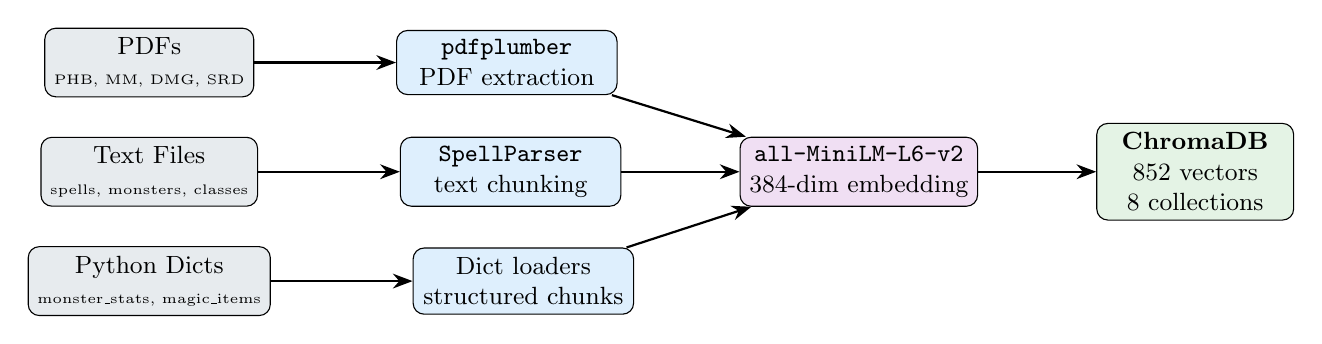
\begin{tikzpicture}[
    node distance=0.5cm and 0.8cm,
    source/.style={draw, rounded corners, fill=layerData!15,
                   minimum width=2.2cm, minimum height=0.7cm,
                   font=\small, align=center},
    process/.style={draw, rounded corners, fill=layerOrch!15,
                    minimum width=2.8cm, minimum height=0.7cm,
                    font=\small, align=center},
    store/.style={draw, rounded corners, fill=layerRAG!15,
                  minimum width=2.5cm, minimum height=0.7cm,
                  font=\small, align=center},
    arrow/.style={-{Stealth[length=2.5mm]}, thick},
]
% Sources column
\node[source] (pdf) {PDFs\\{\tiny PHB, MM, DMG, SRD}};
\node[source, below=of pdf] (txt) {Text Files\\{\tiny spells, monsters, classes}};
\node[source, below=of txt] (dict) {Python Dicts\\{\tiny monster\_stats, magic\_items}};

% Processing column
\node[process, right=1.8cm of pdf] (pdfparse) {\texttt{pdfplumber}\\PDF extraction};
\node[process, right=1.8cm of txt] (spellparse) {\texttt{SpellParser}\\text chunking};
\node[process, right=1.8cm of dict] (dictload) {Dict loaders\\structured chunks};

% Embedding
\node[process, right=1.5cm of spellparse, fill=layerLLM!15]
    (embed) {\texttt{all-MiniLM-L6-v2}\\384-dim embedding};

% Store
\node[store, right=1.5cm of embed]
    (chroma) {\textbf{ChromaDB}\\852 vectors\\8 collections};

% Arrows
\draw[arrow] (pdf) -- (pdfparse);
\draw[arrow] (txt) -- (spellparse);
\draw[arrow] (dict) -- (dictload);
\draw[arrow] (pdfparse) -- (embed);
\draw[arrow] (spellparse) -- (embed);
\draw[arrow] (dictload) -- (embed);
\draw[arrow] (embed) -- (chroma);
\end{tikzpicture}
\caption{ETL pipeline: raw sources are parsed, chunked, embedded, and stored
in ChromaDB.}
\label{fig:etl_pipeline}
\end{figure}

Key processing steps include:
\begin{itemize}[noitemsep]
    \item \textbf{Entity boundary detection}: spells are split on all-caps
          names followed by a level/school line; classes are split on
          all-caps class name headers; monster blocks are identified by
          size-type lines (``Medium humanoid'', etc.).
    \item \textbf{OCR error correction}: common artefacts in the monster and
          class text files (e.g.\ ``S tr e n g t h'') are normalised during
          parsing.
    \item \textbf{Metadata extraction}: challenge ratings, spell levels,
          armour class values, and class--spell associations are extracted via
          regex and stored as ChromaDB metadata.
\end{itemize}

\subsection{Name-Weighted Chunking}
\label{sec:nameweighting}

Standard semantic chunking can fail for proper-noun retrieval because
embedding models prioritise semantic similarity over lexical overlap. For
example, querying ``Goblin'' may return ``Hobgoblin'' first due to shared
descriptive features (Figure~\ref{fig:nameweight}).

\begin{figure}[H]
\centering
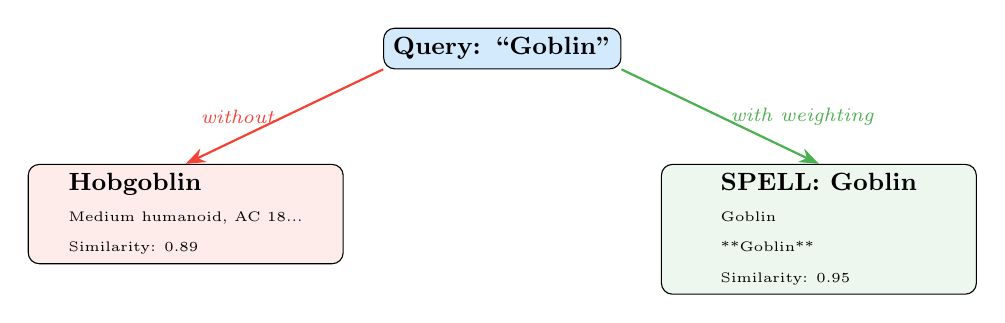
\begin{tikzpicture}[
    node distance=0.6cm,
    chunk/.style={draw, rounded corners, minimum width=4cm,
                  minimum height=1.2cm, font=\small, align=left},
    query/.style={draw, rounded corners, fill=layerOrch!20,
                  minimum width=3cm, font=\small\bfseries},
    arrow/.style={-{Stealth[length=2.5mm]}, thick},
]
% Query
\node[query] (q) {Query: ``Goblin''};

% Without weighting
\node[chunk, below left=1.2cm and 0.5cm of q, fill=failRed!10]
    (bad) {\textbf{Hobgoblin}\\{\tiny Medium humanoid, AC 18...}\\{\tiny Similarity: 0.89}};

% With weighting
\node[chunk, below right=1.2cm and 0.5cm of q, fill=passGreen!10]
    (good) {\textbf{SPELL: Goblin}\\{\tiny Goblin}\\{\tiny **Goblin**}\\{\tiny Similarity: 0.95}};

\draw[arrow, failRed] (q.south west) -- (bad.north)
    node[midway, left, font=\scriptsize\itshape] {without};
\draw[arrow, passGreen] (q.south east) -- (good.north)
    node[midway, right, font=\scriptsize\itshape] {with weighting};
\end{tikzpicture}
\caption{Name-weighted chunking ensures exact entity matches rank first
by repeating the entity name three times in the chunk header.}
\label{fig:nameweight}
\end{figure}

The \texttt{SpellParser} (\texttt{spell\_parser.py}, lines~452--455)
addresses this with a name-weighted template. In the full-spell chunk, the
entity name appears \textbf{three times} within the first few lines:

\begin{lstlisting}[language={},basicstyle=\ttfamily\small,frame=single,numbers=none]
SPELL: Fireball         (* occurrence 1 *)
Fireball                (* occurrence 2 *)
**Fireball**            (* occurrence 3 *)
Level 3 Evocation
...
\end{lstlisting}

This increases the entity name's share of the mean-pooled embedding,
causing the name tokens to dominate the vector direction. A separate
quick-reference chunk (line~496) uses the same weighting pattern.

\subsection{Embedding Model}

\texttt{all-MiniLM-L6-v2}~\cite{reimers2019sbert} (22\,M parameters,
384-dimensional output) is configured in \texttt{settings.py}
(lines~91--94):
\begin{lstlisting}
EMBEDDING_MODEL_NAME = "all-MiniLM-L6-v2"
EMBEDDING_DIMENSION = 384
\end{lstlisting}

It was selected for its speed (${\sim}$2,000 embeddings/s) and small memory
footprint, with quality sufficient given the name-weighting compensation.

\subsection{Vector Database}

ChromaDB~\cite{chromadb} stores the embedded vectors using the HNSW
index~\cite{malkov2018hnsw}. A single initialisation run produces
\textbf{852 vectors} across \textbf{8~collections}
(Table~\ref{tab:collections}), as verified by running the initialisation
script.

\begin{table}[H]
\centering
\caption{ChromaDB collections produced by a single initialisation run.}
\label{tab:collections}
\small
\begin{tabular}{lr}
\toprule
\textbf{Collection} & \textbf{Vectors} \\
\midrule
\texttt{dnd\_spells}       & 586 \\
\texttt{dm\_guide}         & 95 \\
\texttt{dnd\_equipment}    & 60 \\
\texttt{class\_features}   & 38 \\
\texttt{magic\_items}      & 30 \\
\texttt{dnd\_monsters}     & 16 \\
\texttt{dnd\_races}        & 16 \\
\texttt{dnd\_classes}      & 11 \\
\midrule
\textbf{Total}             & \textbf{852} \\
\bottomrule
\end{tabular}
\end{table}

The six primary collections configured in \texttt{settings.py}
(lines~41--48) are \texttt{dnd\_spells}, \texttt{dnd\_monsters},
\texttt{dnd\_classes}, \texttt{dnd\_races}, \texttt{dnd\_equipment}, and
\texttt{dm\_guide}. The initialisation also populates
\texttt{magic\_items} and \texttt{class\_features} via structured Python
dictionaries. Supplementary scripts (SRD parser, Monster Manual PDF
ingestion) can create additional collections such as
\texttt{dnd\_monsters\_v2} and \texttt{dnd5e\_srd}.

% ═════════════════════════════════════════════════════════════════════════
\section{System Architecture}
\label{sec:architecture}

\subsection{Overview}

The system follows a layered architecture (Figure~\ref{fig:architecture}).
User input from the Gradio web UI (\texttt{web/app\_gradio.py}, 903~lines)
or the CLI is routed through a \texttt{GameMaster} facade, which orchestrates
intent classification, reality checking, RAG retrieval, prompt construction,
LLM generation, and game-state updates.

\begin{figure}[H]
\centering
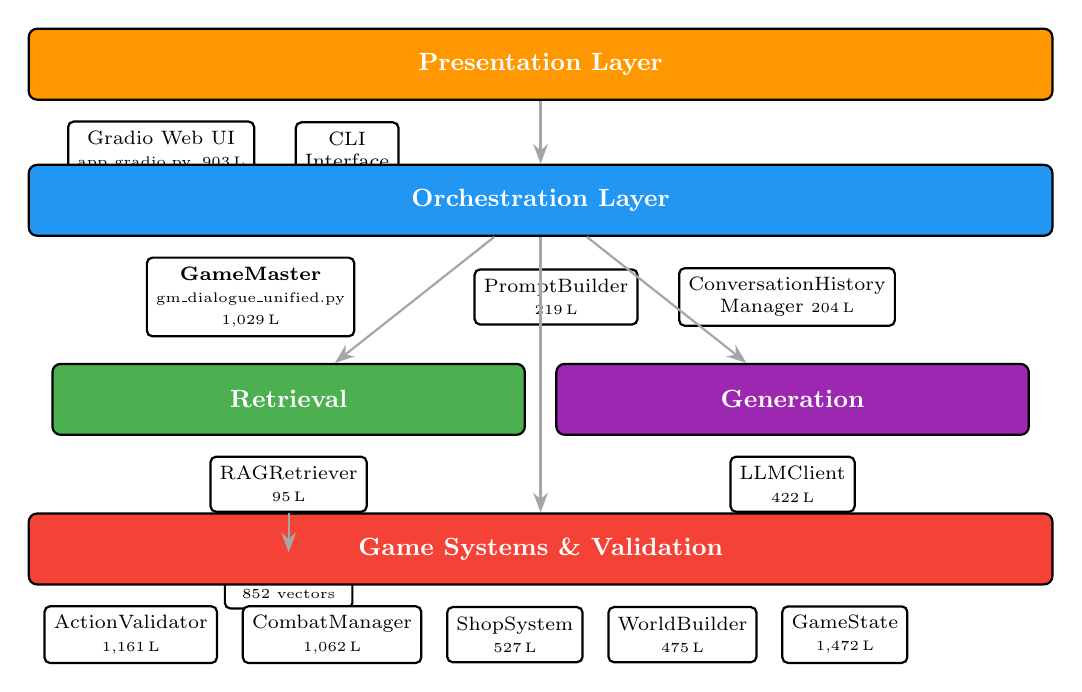
\begin{tikzpicture}[
    node distance=0.4cm and 0.3cm,
    layer/.style={draw, rounded corners=3pt, minimum height=0.9cm,
                  font=\small, align=center, text=white, thick},
    comp/.style={draw, rounded corners=2pt, minimum height=0.7cm,
                 font=\scriptsize, align=center, fill=white, thick},
    arrow/.style={-{Stealth[length=2.5mm]}, thick, gray!70},
]

% ── UI Layer ──
\node[layer, fill=layerUI, minimum width=13cm]
    (ui) {\textbf{Presentation Layer}};
\node[comp, below=0.25cm of ui.south west, anchor=north west, xshift=0.5cm]
    (gradio) {Gradio Web UI\\{\tiny app\_gradio.py, 903\,L}};
\node[comp, right=0.5cm of gradio]
    (cli) {CLI\\Interface};

% ── Orchestration Layer ──
\node[layer, fill=layerOrch, minimum width=13cm,
      below=0.8cm of ui]
    (orch) {\textbf{Orchestration Layer}};
\node[comp, below=0.25cm of orch.south west, anchor=north west, xshift=1.5cm]
    (gm) {\textbf{GameMaster}\\{\tiny gm\_dialogue\_unified.py}\\{\tiny 1,029\,L}};
\node[comp, right=1.5cm of gm]
    (prompt) {PromptBuilder\\{\tiny 219\,L}};
\node[comp, right=0.5cm of prompt]
    (conv) {ConversationHistory\\Manager {\tiny 204\,L}};

% ── Retrieval + Generation Layer ──
\node[layer, fill=layerRAG, minimum width=6cm,
      below=1.6cm of orch.south west, anchor=north west, xshift=0.3cm]
    (retlayer) {\textbf{Retrieval}};
\node[layer, fill=layerLLM, minimum width=6cm,
      below=1.6cm of orch.south east, anchor=north east, xshift=-0.3cm]
    (genlayer) {\textbf{Generation}};

\node[comp, below=0.25cm of retlayer]
    (rag) {RAGRetriever\\{\tiny 95\,L}};
\node[comp, below=0.25cm of genlayer]
    (llm) {LLMClient\\{\tiny 422\,L}};
\node[comp, below=0.5cm of rag]
    (chroma) {ChromaDB\\{\tiny 852 vectors}};

% ── Validation + Game Systems Layer ──
\node[layer, fill=layerState, minimum width=13cm,
      below=3.5cm of orch]
    (statelayer) {\textbf{Game Systems \& Validation}};

\node[comp, below=0.25cm of statelayer.south west, anchor=north west,
      xshift=0.2cm]
    (av) {ActionValidator\\{\tiny 1,161\,L}};
\node[comp, right=0.3cm of av]
    (combat) {CombatManager\\{\tiny 1,062\,L}};
\node[comp, right=0.3cm of combat]
    (shop) {ShopSystem\\{\tiny 527\,L}};
\node[comp, right=0.3cm of shop]
    (world) {WorldBuilder\\{\tiny 475\,L}};
\node[comp, right=0.3cm of world]
    (gs) {GameState\\{\tiny 1,472\,L}};

% ── Arrows ──
\draw[arrow] (ui) -- (orch);
\draw[arrow] (orch) -- (retlayer);
\draw[arrow] (orch) -- (genlayer);
\draw[arrow] (orch) -- (statelayer);
\draw[arrow] (rag) -- (chroma);
\end{tikzpicture}
\caption{Layered system architecture with component line counts.
Colours encode functional layers: \textcolor{layerUI}{presentation},
\textcolor{layerOrch}{orchestration},
\textcolor{layerRAG}{retrieval},
\textcolor{layerLLM}{generation},
\textcolor{layerState}{game systems}.}
\label{fig:architecture}
\end{figure}

The \texttt{dnd\_rag\_system/} package totals approximately 19,000 lines
across 56 Python files. Including tests, scripts, and the web interface, the
full project contains 233 Python files.

The architecture emerged through seven incremental refactoring phases
(documented in \texttt{docs/REFACTORING\_SUMMARY.md}) that decomposed an
initial monolithic \texttt{GameMaster} class into the current set of
focused components.

\subsection{RAG Pipeline}
\label{sec:ragpipeline}

The RAG pipeline processes each player turn in six stages
(Figure~\ref{fig:rag_sequence}):

\begin{figure}[H]
\centering
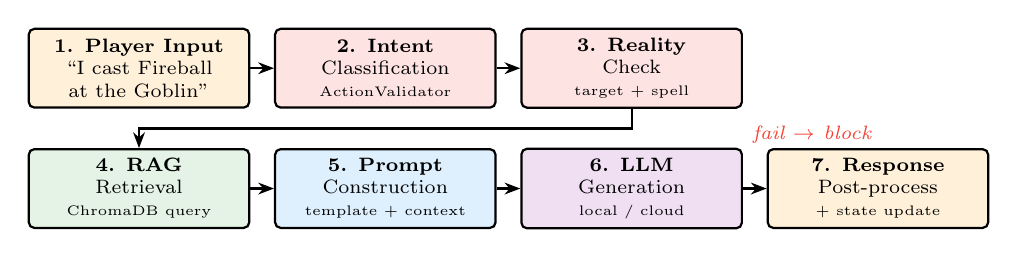
\begin{tikzpicture}[
    node distance=0.15cm,
    stage/.style={draw, rounded corners=2pt, minimum width=2.8cm,
                  minimum height=1cm, font=\scriptsize, align=center,
                  thick},
    arrow/.style={-{Stealth[length=2mm]}, thick},
]
% Stages in a flow
\node[stage, fill=layerUI!15] (s1) {\textbf{1. Player Input}\\``I cast Fireball\\at the Goblin''};
\node[stage, fill=layerState!15, right=0.3cm of s1]
    (s2) {\textbf{2. Intent}\\Classification\\{\tiny ActionValidator}};
\node[stage, fill=layerState!15, right=0.3cm of s2]
    (s3) {\textbf{3. Reality}\\Check\\{\tiny target + spell}};
\node[stage, fill=layerRAG!15, below=0.5cm of s1]
    (s4) {\textbf{4. RAG}\\Retrieval\\{\tiny ChromaDB query}};
\node[stage, fill=layerOrch!15, right=0.3cm of s4]
    (s5) {\textbf{5. Prompt}\\Construction\\{\tiny template + context}};
\node[stage, fill=layerLLM!15, right=0.3cm of s5]
    (s6) {\textbf{6. LLM}\\Generation\\{\tiny local / cloud}};
\node[stage, fill=layerUI!15, right=0.3cm of s6]
    (s7) {\textbf{7. Response}\\Post-process\\{\tiny + state update}};

\draw[arrow] (s1) -- (s2);
\draw[arrow] (s2) -- (s3);
\draw[arrow] (s3.south) -- ++(0,-0.25) -| (s4.north);
\draw[arrow] (s4) -- (s5);
\draw[arrow] (s5) -- (s6);
\draw[arrow] (s6) -- (s7);

% Fail path
\node[font=\scriptsize\itshape, text=failRed, below=0.1cm of s3.south east,
      anchor=north west] {fail $\rightarrow$ block};
\end{tikzpicture}
\caption{RAG pipeline sequence for a single player turn.  If the Reality
Check (stage~3) fails, the LLM is bypassed and a deterministic error is
returned.}
\label{fig:rag_sequence}
\end{figure}

\begin{enumerate}[noitemsep]
    \item \textbf{Intent classification} (\texttt{ActionValidator},
          1,161~lines): a keyword-based classifier identifies the action type
          (attack, spell, shop, travel, etc.). An optional LLM-based fallback
          handles creative phrasings such as ``loose an arrow''
          $\rightarrow$ \textsc{attack}.
    \item \textbf{Reality Check}: the target and action are validated against
          the in-memory game state (Section~\ref{sec:realitycheck}).
    \item \textbf{RAG retrieval} (\texttt{RAGRetriever}, 95~lines): the
          extracted entity name is embedded and queried against the ChromaDB
          collections.
    \item \textbf{Prompt construction} (\texttt{PromptBuilder}, 219~lines): a
          template is populated with character context, retrieved rules,
          conversation summary, recent messages, and the player input.
    \item \textbf{LLM generation} (\texttt{LLMClient}, 422~lines): the prompt
          is sent to Ollama (local) or HuggingFace (cloud). Default parameters
          (\texttt{llm\_client.py}): \texttt{temperature\,=\,0.7},
          \texttt{top\_p\,=\,0.9}, \texttt{max\_tokens\,=\,300}.
    \item \textbf{Post-processing}: thinking tokens are stripped,
          game-mechanic values (damage, HP changes) are extracted via regex,
          and the game state is updated.
\end{enumerate}

\subsection{LLM Selection}
\label{sec:llm}

The primary model is \textbf{Qwen3-4B}~\cite{bai2023qwen}, a
4-billion-parameter model quantised to Q4\_K\_M (${\sim}$2.8\,GB). It was
chosen for its narrative coherence while fitting within the 16\,GB RAM limit
of HuggingFace Spaces.

A dual-backend architecture (\texttt{llm\_client.py}) supports automatic
fallback (Figure~\ref{fig:deployment}):
\begin{itemize}[noitemsep]
    \item \textbf{Ollama} (local): connects to \texttt{localhost:11434}.
    \item \textbf{HuggingFace Inference API}: activates automatically when
          the \texttt{SPACE\_ID} environment variable is detected. Uses
          Qwen2.5-7B-Instruct.
\end{itemize}

\subsection{Reality Check System}
\label{sec:realitycheck}

The Reality Check is a \emph{deterministic} validation layer in
\texttt{ActionValidator} (1,161~lines) that runs \emph{before} the LLM
generates a response. Figure~\ref{fig:realitycheck} shows the decision
flow.

\begin{figure}[H]
\centering
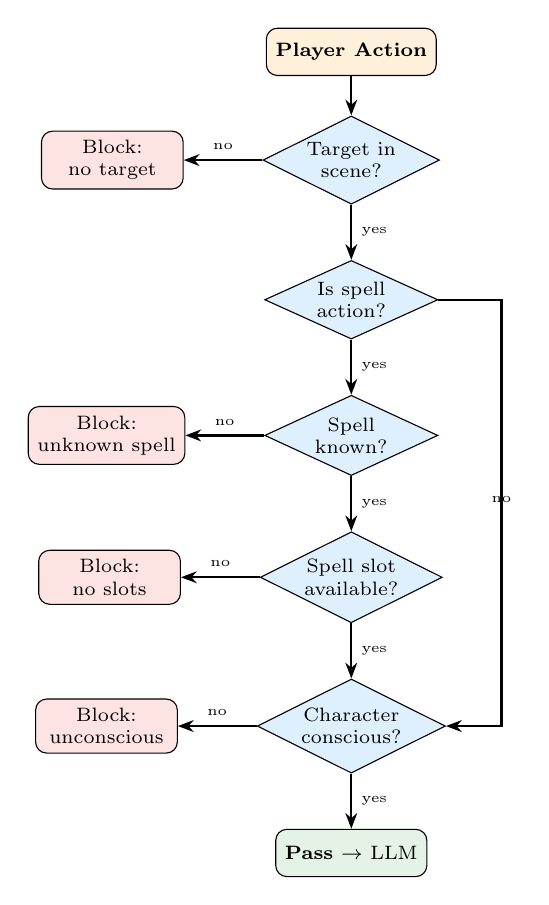
\begin{tikzpicture}[
    node distance=0.6cm,
    decision/.style={draw, diamond, aspect=2, fill=layerOrch!15,
                     font=\scriptsize, align=center, inner sep=1pt,
                     minimum width=2.2cm},
    block/.style={draw, rounded corners, fill=failRed!15,
                  font=\scriptsize, align=center,
                  minimum width=1.8cm, minimum height=0.6cm},
    pass/.style={draw, rounded corners, fill=passGreen!15,
                 font=\scriptsize, align=center,
                 minimum width=1.8cm, minimum height=0.6cm},
    input/.style={draw, rounded corners, fill=layerUI!15,
                  font=\scriptsize\bfseries, align=center,
                  minimum width=2cm, minimum height=0.6cm},
    arrow/.style={-{Stealth[length=2mm]}, thick},
]
\node[input] (in) {Player Action};
\node[decision, below=0.5cm of in] (d1) {Target in\\scene?};
\node[block, left=1cm of d1] (b1) {Block:\\no target};
\node[decision, below=0.7cm of d1] (d2) {Is spell\\action?};
\node[decision, below=0.7cm of d2] (d3) {Spell\\known?};
\node[block, left=1cm of d3] (b3) {Block:\\unknown spell};
\node[decision, below=0.7cm of d3] (d4) {Spell slot\\available?};
\node[block, left=1cm of d4] (b4) {Block:\\no slots};
\node[decision, below=0.7cm of d4] (d5) {Character\\conscious?};
\node[block, left=1cm of d5] (b5) {Block:\\unconscious};
\node[pass, below=0.7cm of d5] (ok) {\textbf{Pass} $\rightarrow$ LLM};

\draw[arrow] (in) -- (d1);
\draw[arrow] (d1) -- node[above,font=\tiny]{no} (b1);
\draw[arrow] (d1) -- node[right,font=\tiny]{yes} (d2);
\draw[arrow] (d2) -- node[right,font=\tiny]{yes} (d3);
\draw[arrow] (d2.east) -- ++(0.8,0) |- node[near start,above,font=\tiny]{no} (d5);
\draw[arrow] (d3) -- node[above,font=\tiny]{no} (b3);
\draw[arrow] (d3) -- node[right,font=\tiny]{yes} (d4);
\draw[arrow] (d4) -- node[above,font=\tiny]{no} (b4);
\draw[arrow] (d4) -- node[right,font=\tiny]{yes} (d5);
\draw[arrow] (d5) -- node[above,font=\tiny]{no} (b5);
\draw[arrow] (d5) -- node[right,font=\tiny]{yes} (ok);
\end{tikzpicture}
\caption{Reality Check decision flowchart. Each red block prevents
hallucination by returning a deterministic error \emph{without} invoking
the LLM.}
\label{fig:realitycheck}
\end{figure}

The checks include:
\begin{itemize}[noitemsep]
    \item \textbf{Target validation} (lines~334--407): the named target must
          exist in the current scene. Fuzzy matching handles articles and
          casing.
    \item \textbf{Spell validation} (lines~453--537): the character must
          know the spell and have an available spell slot of the required
          level.
    \item \textbf{Inventory validation} (lines~337--350): weapons and items
          referenced must be in the character's inventory.
    \item \textbf{Combat-state validation}: attack actions require active
          combat; unconscious characters cannot act.
\end{itemize}

If validation fails, a deterministic error message is returned without
invoking the LLM. This eliminates entire categories of hallucination
(Section~\ref{sec:hallucination}).

\subsection{Context Window Management}

The \texttt{ConversationHistoryManager} (204~lines) caps conversation history
at \textbf{20~messages} (\texttt{MAX\_MESSAGE\_HISTORY\,=\,20} in
\texttt{settings.py}). Only the \textbf{10 most recent messages} are
included in the LLM prompt (\texttt{RECENT\_MESSAGES\_FOR\_PROMPT\,=\,10}).
Older messages are summarised to preserve long-term narrative continuity
while preventing context-window overflow and latency degradation.

\subsection{Prompt Template System}

All LLM prompts are externalised to \textbf{nine} template files in
\texttt{dnd\_rag\_system/prompts/}:
\texttt{mechanics\_extraction},
\texttt{intent\_classification},
\texttt{explore\_location},
\texttt{monster\_encounter},
\texttt{multi\_monster\_encounter},
\texttt{item\_lore},
\texttt{validation\_no\_target},
\texttt{validation\_no\_spell\_slots}, and
\texttt{validation\_invalid\_action}.
Templates use Python string formatting with named variables, separating
prompt engineering from application logic.

\subsection{Game Subsystems}

Beyond the core RAG pipeline, the system implements several D\&D mechanics.
The game transitions between modes as shown in
Figure~\ref{fig:statemachine}.

\begin{figure}[H]
\centering
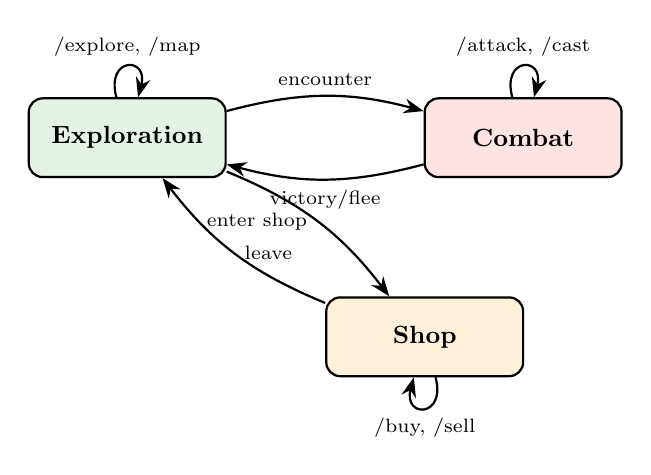
\begin{tikzpicture}[
    node distance=2.5cm,
    state/.style={draw, rounded corners=5pt, minimum width=2.5cm,
                  minimum height=1cm, font=\small\bfseries,
                  align=center, thick},
    arrow/.style={-{Stealth[length=2.5mm]}, thick},
]
\node[state, fill=layerRAG!15]   (explore) {Exploration};
\node[state, fill=layerState!15, right=of explore] (combat) {Combat};
\node[state, fill=layerUI!15, below right=1.5cm and 1.25cm of explore] (shop) {Shop};

\draw[arrow, bend left=15] (explore) to
    node[above, font=\scriptsize] {encounter} (combat);
\draw[arrow, bend left=15] (combat) to
    node[below, font=\scriptsize] {victory/flee} (explore);
\draw[arrow, bend left=15] (explore) to
    node[left, font=\scriptsize] {enter shop} (shop);
\draw[arrow, bend left=15] (shop) to
    node[right, font=\scriptsize] {leave} (explore);

\draw[arrow, loop above, looseness=5] (explore) to
    node[above, font=\scriptsize] {/explore, /map} (explore);
\draw[arrow, loop above, looseness=5] (combat) to
    node[above, font=\scriptsize] {/attack, /cast} (combat);
\draw[arrow, loop below, looseness=5] (shop) to
    node[below, font=\scriptsize] {/buy, /sell} (shop);
\end{tikzpicture}
\caption{Game state machine.  The system transitions between exploration,
combat, and shop modes based on player actions and game events.}
\label{fig:statemachine}
\end{figure}

\begin{description}[noitemsep]
    \item[Combat] (\texttt{combat\_manager.py}, 1,062~lines): turn-based
        combat with initiative tracking, attack rolls, damage calculation,
        and HP management.
    \item[Shop] (\texttt{shop\_system.py}, 527~lines): conversational
        NPC-driven shopping with \texttt{attempt\_purchase()},
        \texttt{attempt\_sale()}, gold tracking, and natural-language
        purchase intent parsing.
    \item[World] (\texttt{world\_builder.py}, 475~lines): procedural
        location generation via \texttt{generate\_random\_location()} with
        weighted type transitions (e.g.\ forests lead to caves with
        weight~0.3, ruins~0.2, more forest~0.25).
    \item[Character creation] (\texttt{character\_creator.py}, 495~lines):
        RAG-powered creation applying racial bonuses, class features, hit
        dice, and spell slots for levels~1--20.
    \item[Game state] (\texttt{game\_state.py}, 1,472~lines):
        \texttt{GameSession} class managing world map, location
        visits, character state, inventory, and combat tracking.
    \item[Spell management] (\texttt{spell\_manager.py}, 407~lines): spell
        lookup, CR-to-XP conversion, and spell slot tracking.
    \item[Magic items] (\texttt{magic\_item\_manager.py}): 30~magic items
        with attunement limits (max~3), slot management, and automatic
        stat bonuses.
\end{description}

% ═════════════════════════════════════════════════════════════════════════
\section{User Interface}
\label{sec:ui}

The Gradio web interface (\texttt{web/app\_gradio.py}, 903~lines) provides
three main tabs: \emph{Play Game}, \emph{Create Character}, and
\emph{Party Management}.

\subsection{Gameplay Interface}

Figure~\ref{fig:gameplay} shows the main gameplay screen.  The left panel
allows character selection from pre-made characters (Thorin
Stormshield---Dwarf Fighter, Elara Moonwhisper---Elf Wizard) or custom
characters, with an optional debug scenario selector.  The right panel
displays the Game Session chat, where the AI GM narrates the adventure and
responds to player actions.

\begin{figure}[H]
\centering
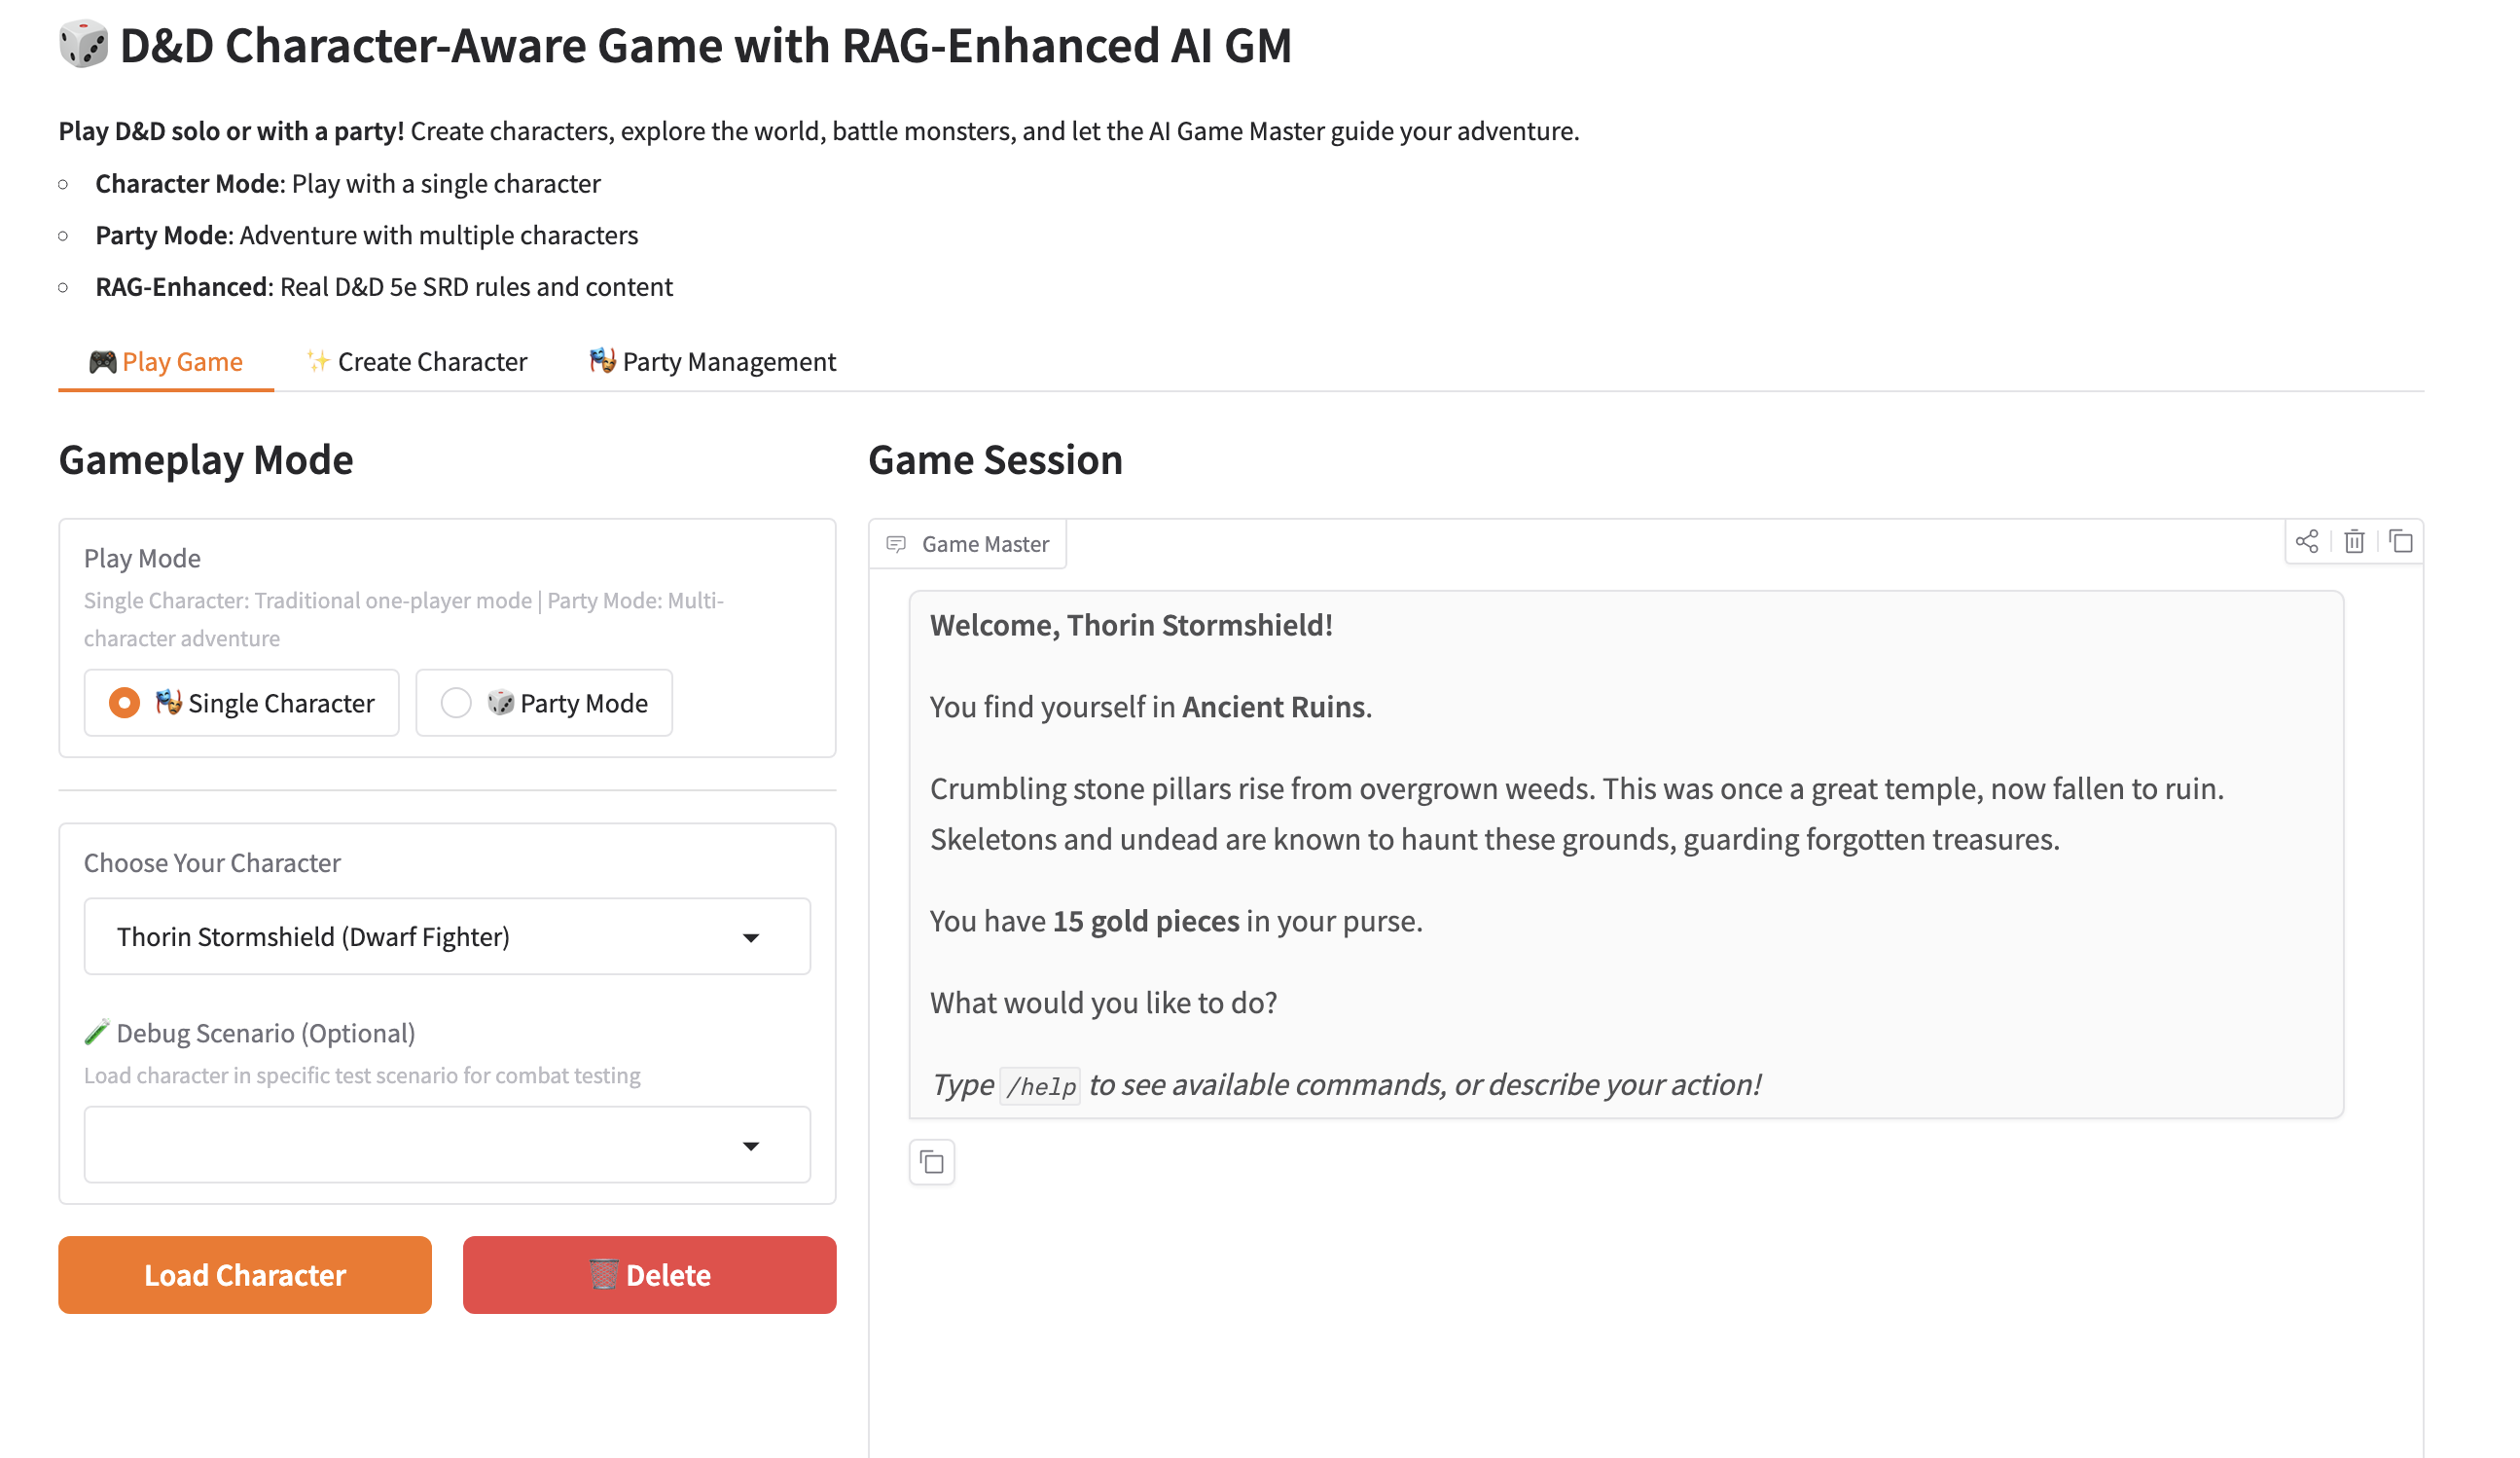
\includegraphics[width=\textwidth]{screenshot_gameplay.png}
\caption{Main gameplay interface showing character selection (left) and
the Game Session chat with the AI GM (right).  The welcome message
introduces the location, describes the environment, and prompts for the
first action.}
\label{fig:gameplay}
\end{figure}

\subsection{Character Sheet}

Below the chat, a live character sheet (Figure~\ref{fig:charsheet}) displays
combat stats (HP, AC, proficiency bonus, gold, XP), ability scores,
equipment, class features, and inventory.  Action buttons (\emph{Attack},
\emph{Cast Spell}, \emph{Use Item}, \emph{Help}) and quick slash commands
(\texttt{/help}, \texttt{/stats}, \texttt{/map}, \texttt{/explore},
\texttt{/buy}, \texttt{/sell}) provide shortcuts.

\begin{figure}[H]
\centering
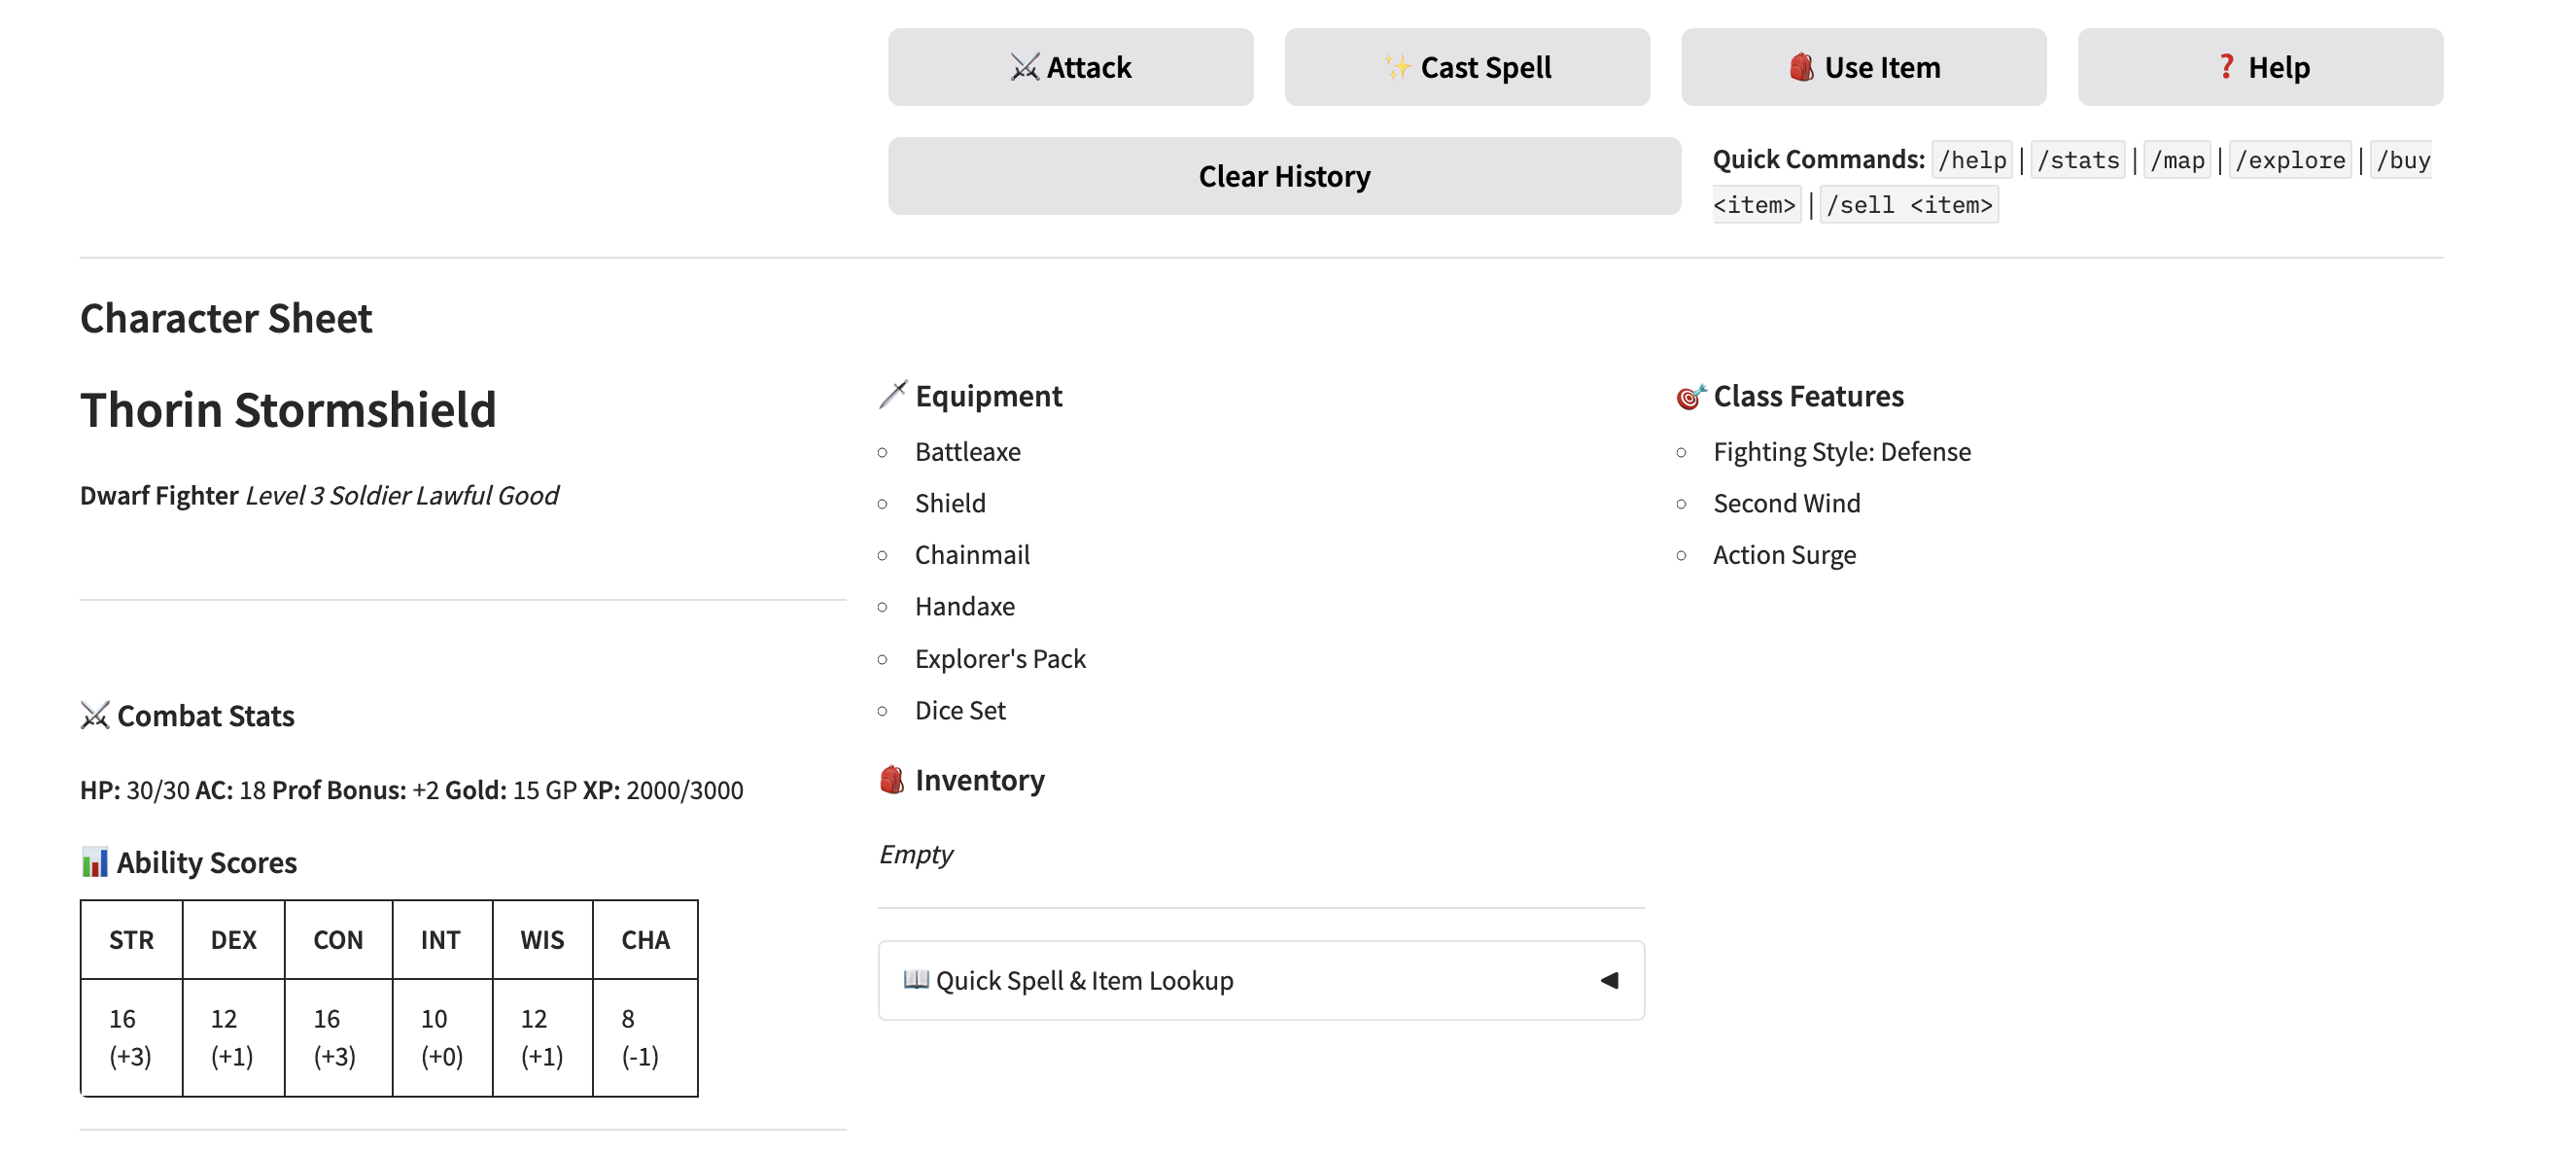
\includegraphics[width=\textwidth]{screenshot_charsheet.png}
\caption{Character sheet for Thorin Stormshield (Dwarf Fighter, Level~3)
showing combat stats, ability scores, equipment, class features, and
action buttons.}
\label{fig:charsheet}
\end{figure}

\subsection{Spell Slot Tracking}

For spellcasting characters, the character sheet
(Figure~\ref{fig:spellsheet}) tracks spell slots per level with a visual
indicator, lists all known spells by level, and shows auto-prepared spells.
A \emph{Quick Spell \& Item Lookup} panel provides direct RAG search.

\begin{figure}[H]
\centering
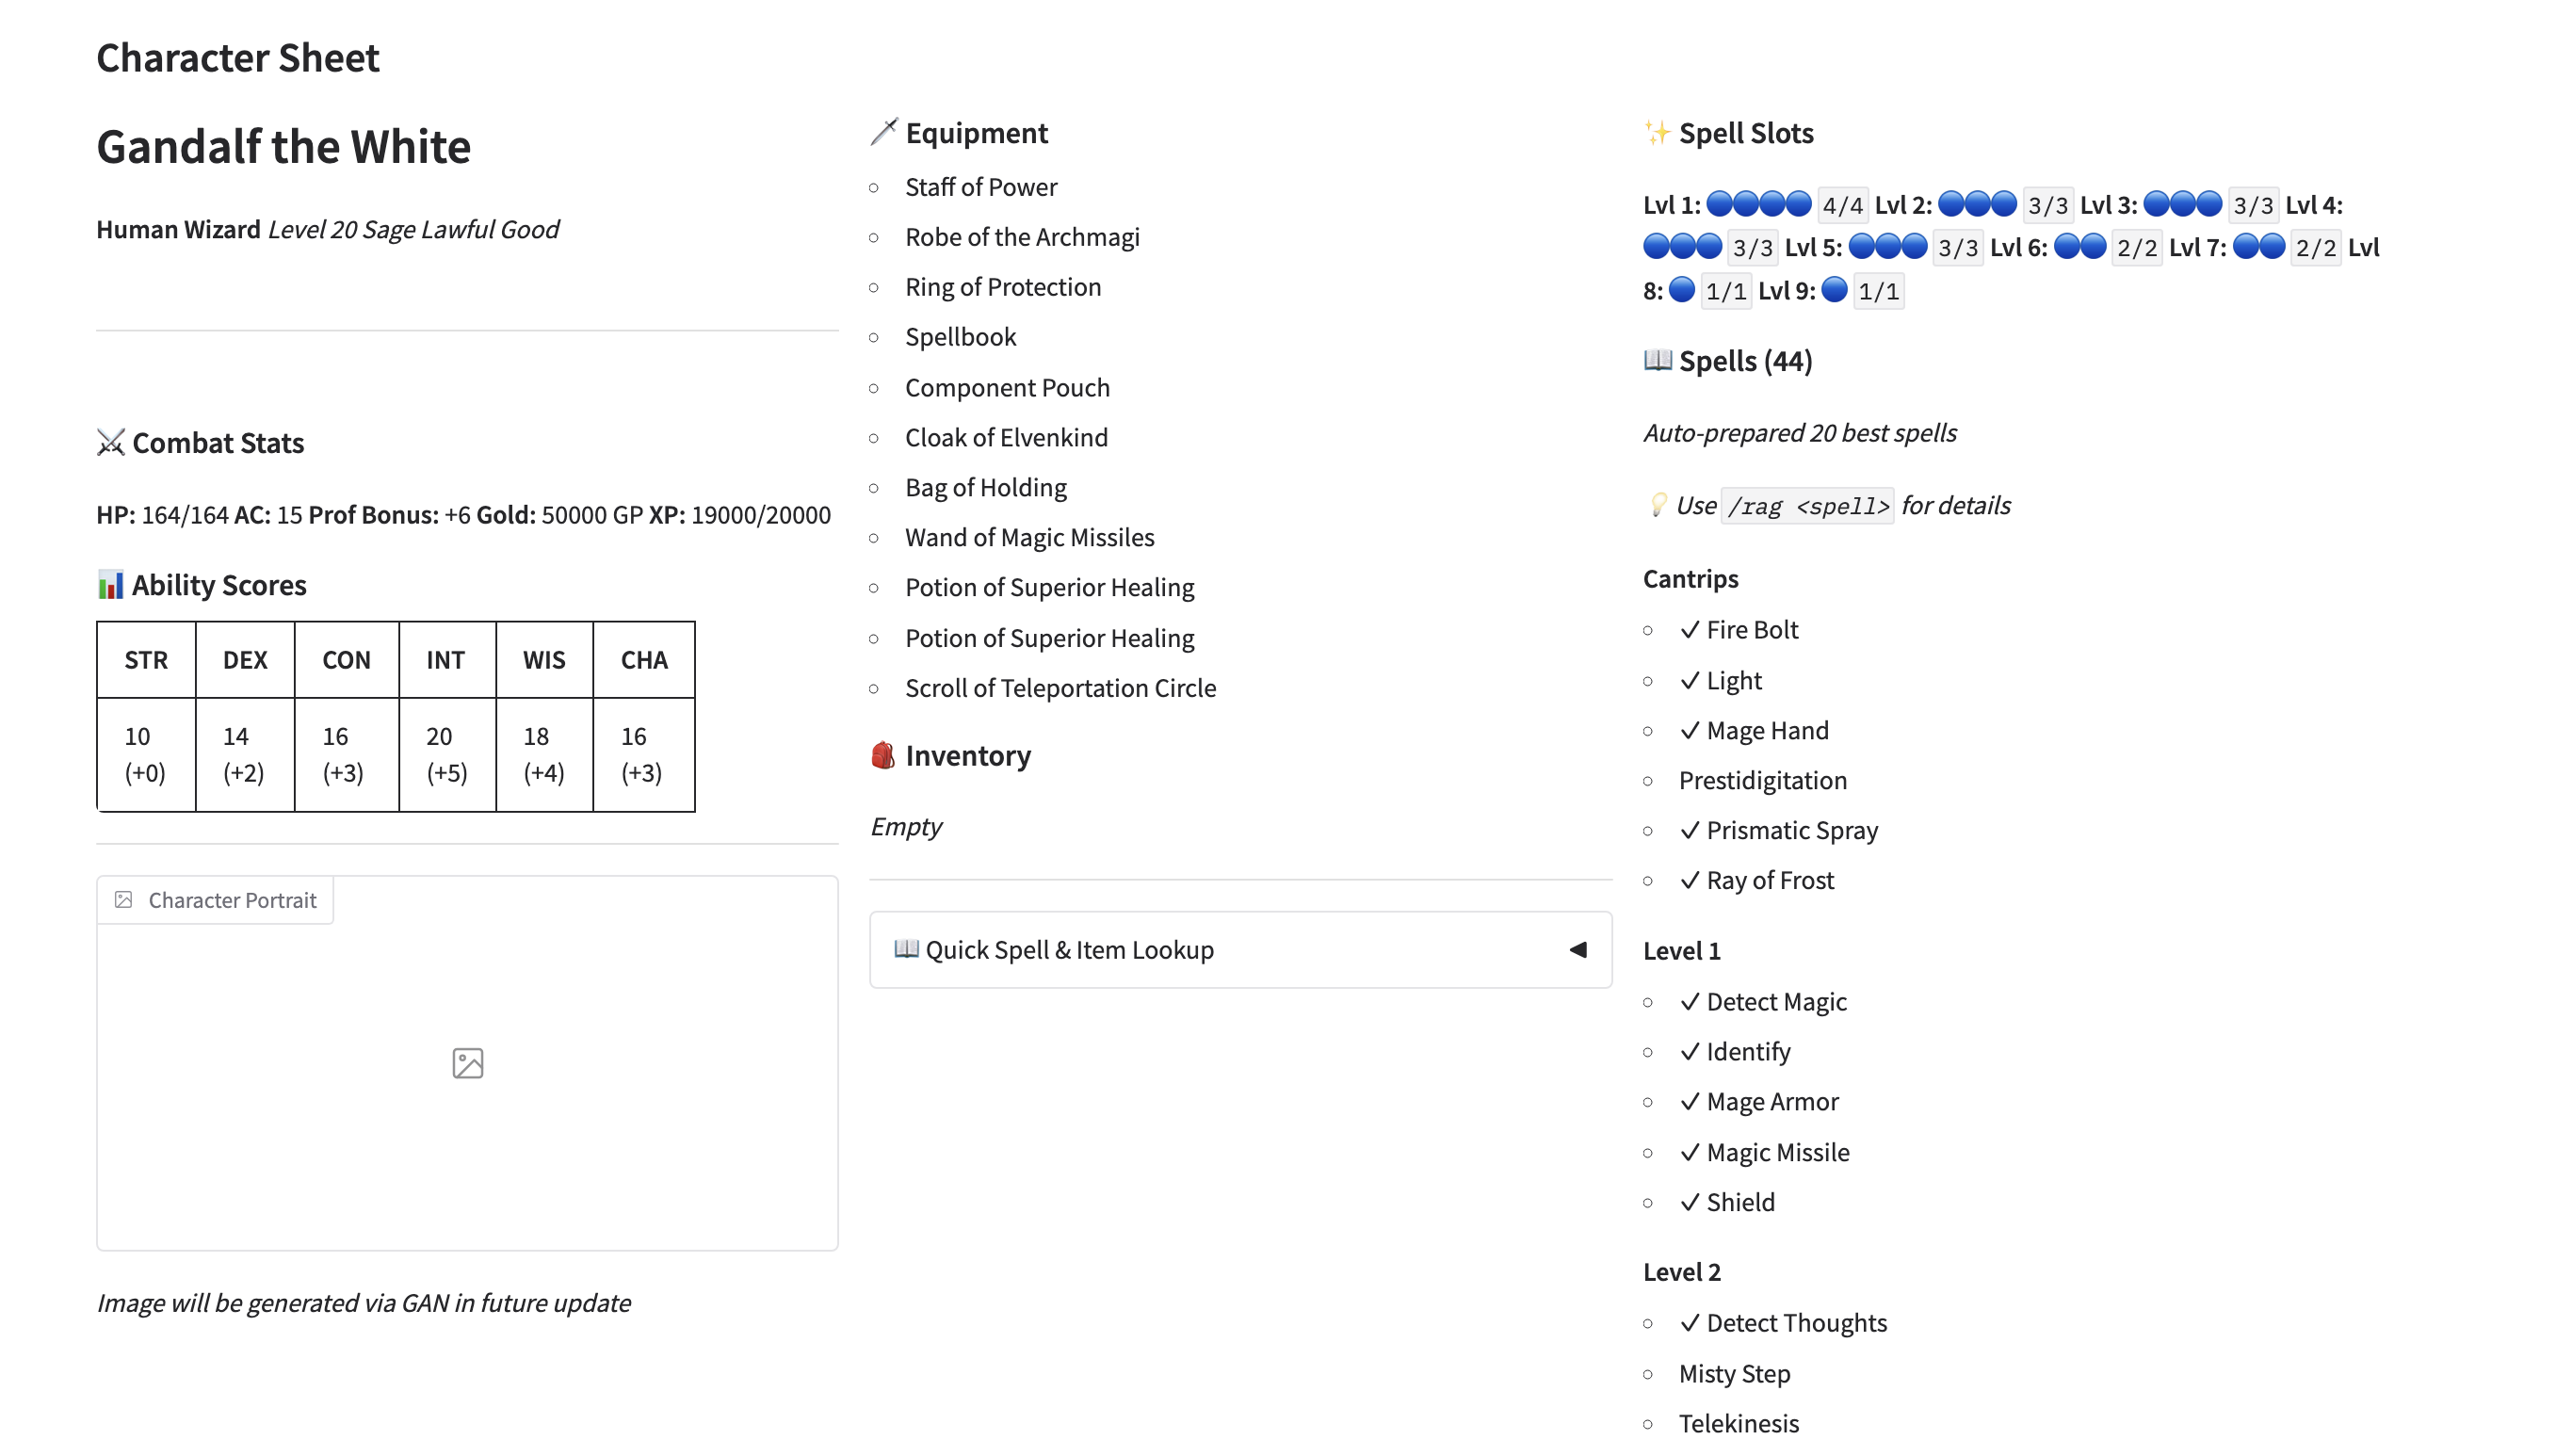
\includegraphics[width=\textwidth]{screenshot_spells.png}
\caption{Character sheet for Gandalf the White (Human Wizard, Level~20)
showing spell slot tracking across levels~1--9, the full spell list (44
spells), equipment including magic items, and the RAG lookup panel.}
\label{fig:spellsheet}
\end{figure}

\subsection{Character Creation}

The \emph{Create Character} tab (Figure~\ref{fig:charcreate}) provides
fields for character name, race (9~PHB races), class (12~PHB classes),
level~(1--20), alignment, and background. Ability scores can be assigned
manually via sliders or rolled randomly (3d6). The standard array
(15, 14, 13, 12, 10, 8) is also offered.

\begin{figure}[H]
\centering
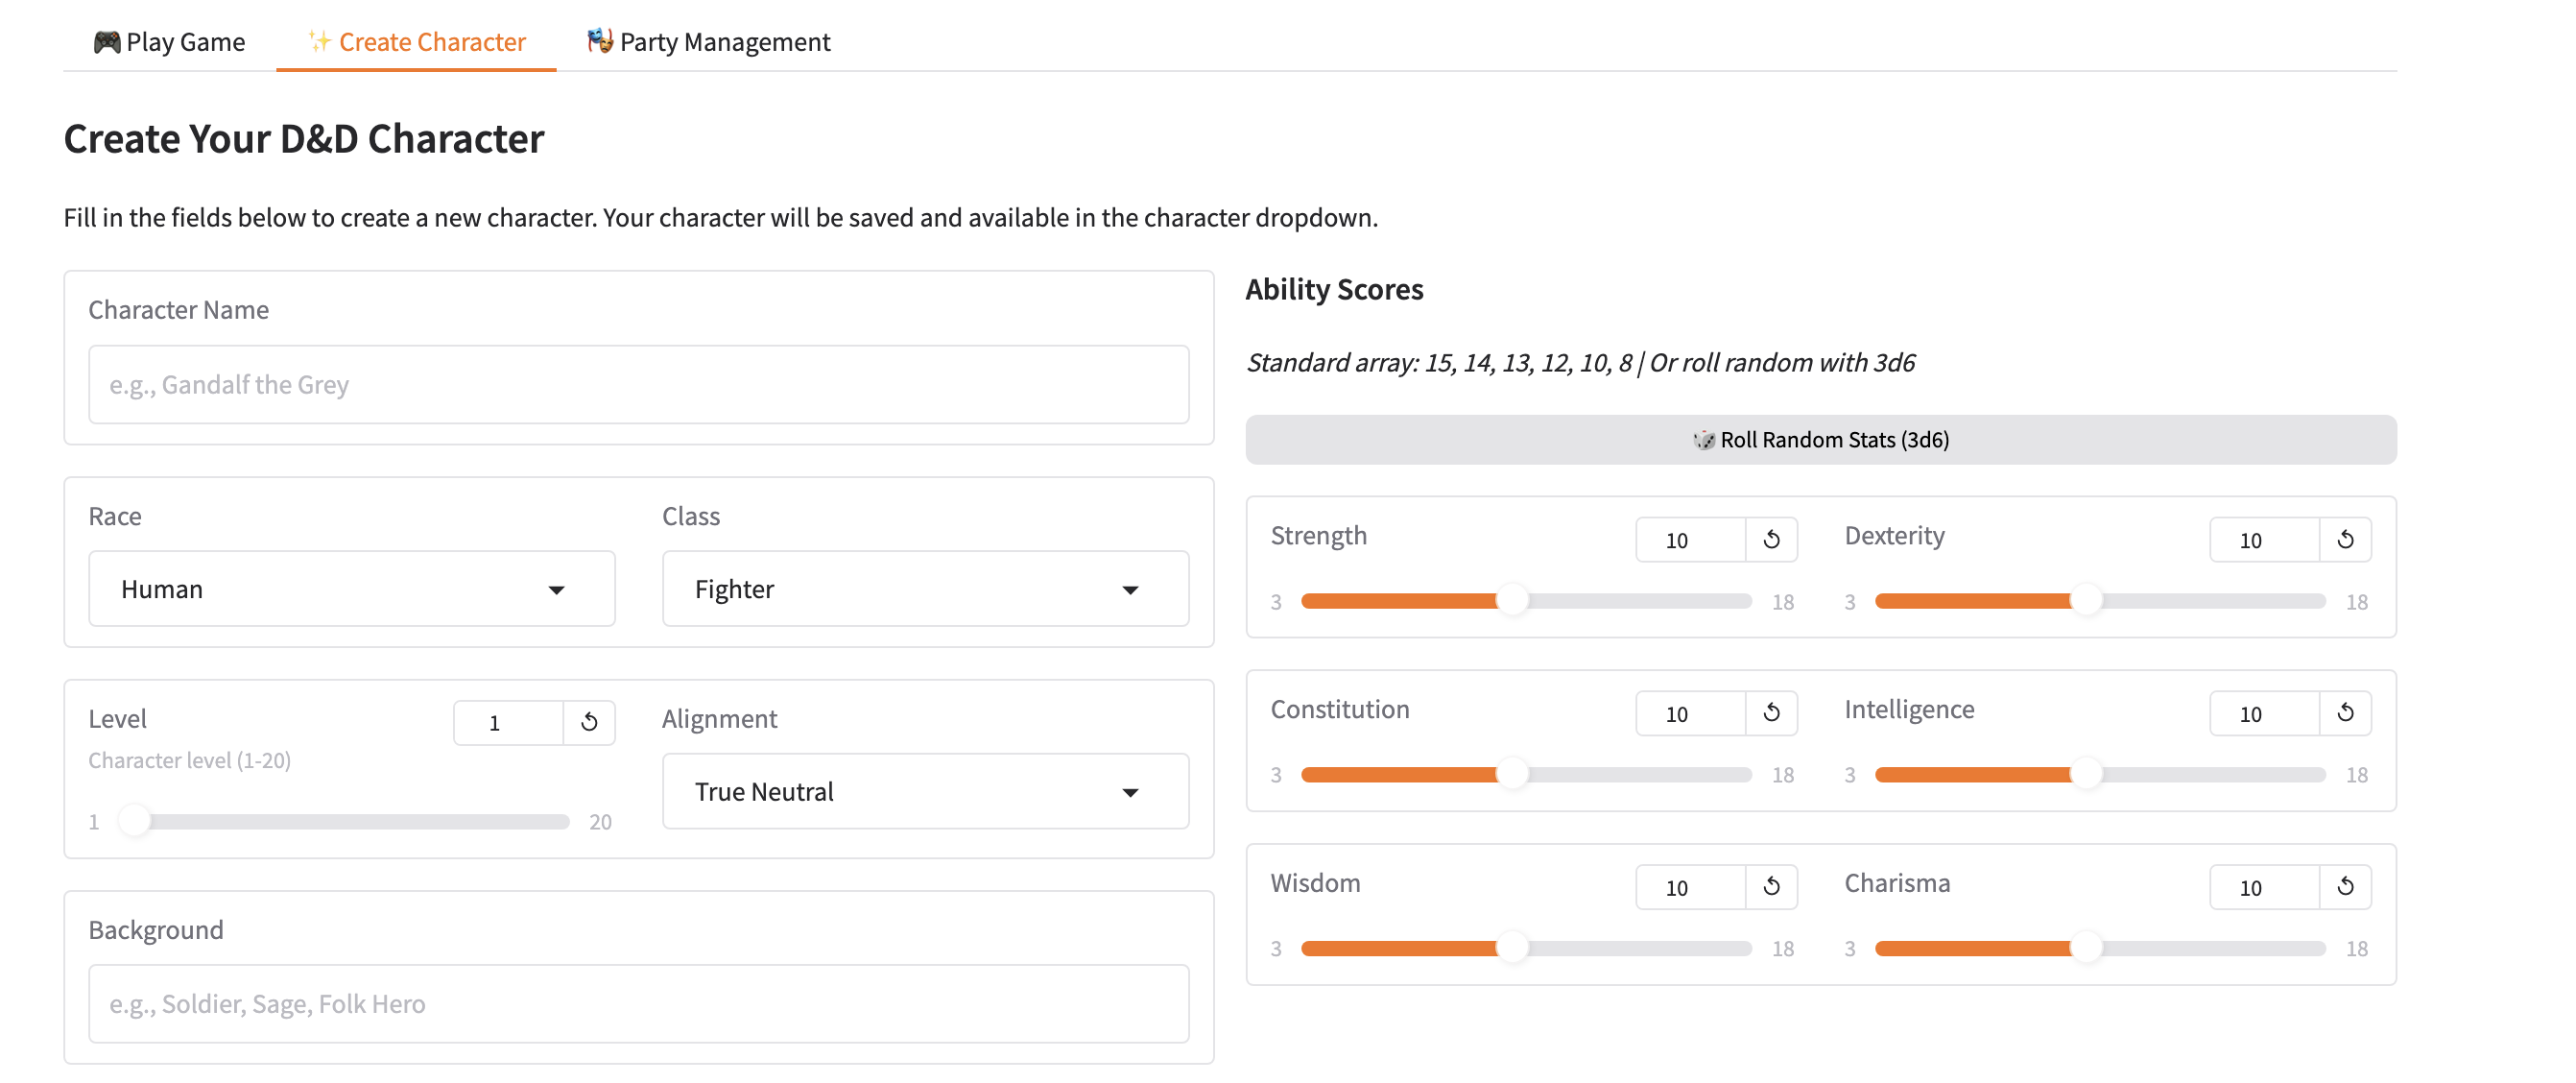
\includegraphics[width=\textwidth]{screenshot_charcreate.png}
\caption{Character creation interface with race/class selectors, level
slider (1--20), alignment dropdown, and ability score sliders with random
roll option.}
\label{fig:charcreate}
\end{figure}

\subsection{Party Management}

The \emph{Party Management} tab (Figure~\ref{fig:party}) enables
multi-character adventures.  Players can assemble a party from pre-made and
custom characters, view a party overview with individual character stats,
and manage party composition. Party members share gold and interact in the
same game session.

\begin{figure}[H]
\centering
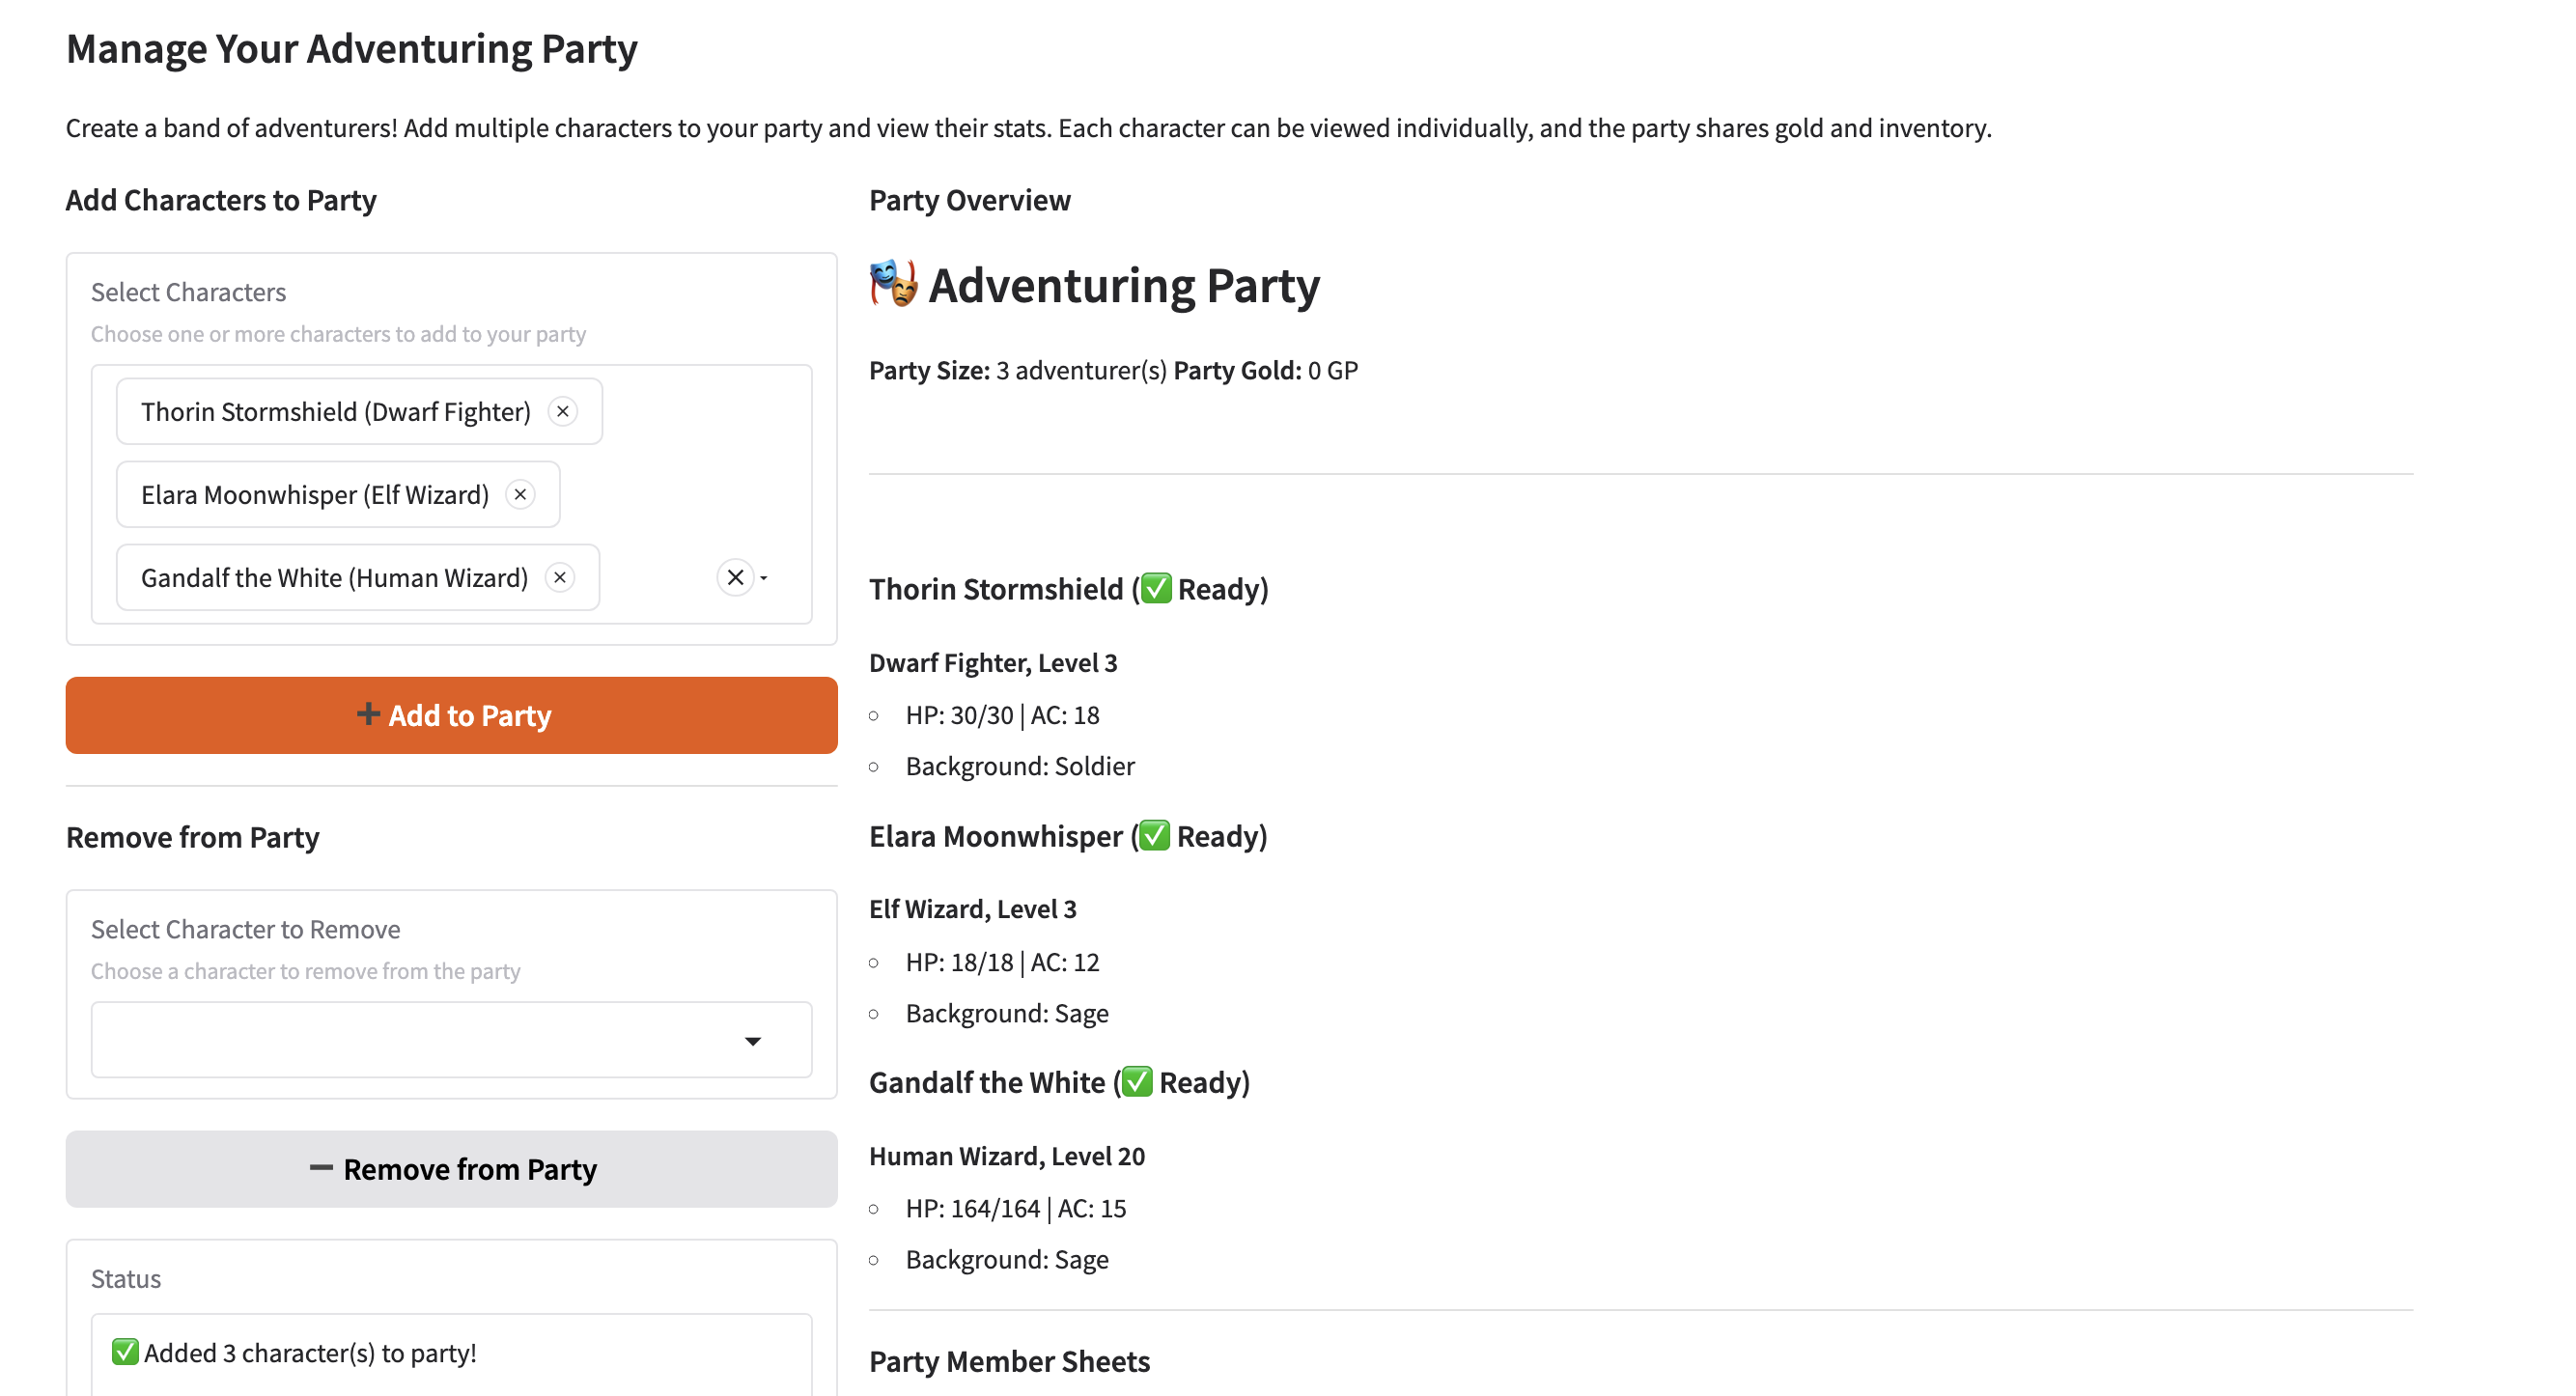
\includegraphics[width=\textwidth]{screenshot_party.png}
\caption{Party management interface showing a 3-character adventuring party
with individual stat summaries (HP, AC, level, background).}
\label{fig:party}
\end{figure}

% ═════════════════════════════════════════════════════════════════════════
\section{Deployment}
\label{sec:deployment}

The system is deployed on \textbf{HuggingFace Spaces} using Docker
(\texttt{Dockerfile}, \texttt{docker-compose.yml}).
Figure~\ref{fig:deployment} shows the dual deployment architecture.

\begin{figure}[H]
\centering
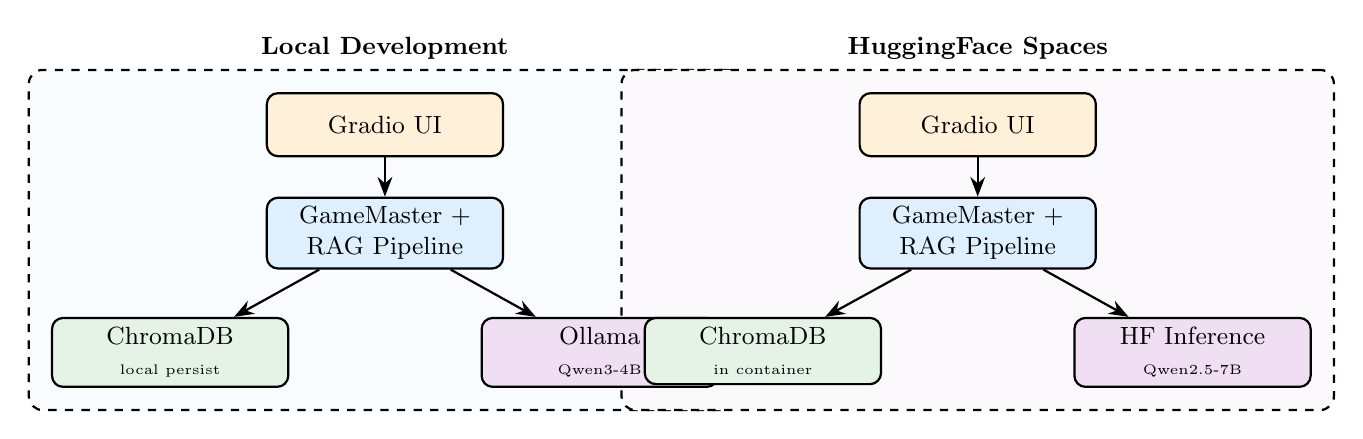
\begin{tikzpicture}[
    node distance=0.5cm and 1.5cm,
    box/.style={draw, rounded corners, minimum width=3cm,
                minimum height=0.8cm, font=\small, align=center, thick},
    env/.style={draw, dashed, rounded corners=5pt, inner sep=8pt,
                thick},
    arrow/.style={-{Stealth[length=2.5mm]}, thick},
]
% Local
\node[box, fill=layerUI!15] (lgrad) {Gradio UI};
\node[box, fill=layerOrch!15, below=of lgrad] (lgm) {GameMaster +\\RAG Pipeline};
\node[box, fill=layerRAG!15, below left=0.6cm and -0.3cm of lgm]
    (lchroma) {ChromaDB\\{\tiny local persist}};
\node[box, fill=layerLLM!15, below right=0.6cm and -0.3cm of lgm]
    (lollama) {Ollama\\{\tiny Qwen3-4B}};

\begin{scope}[on background layer]
\node[env, fill=layerOrch!3,
      fit=(lgrad)(lgm)(lchroma)(lollama),
      label={[font=\small\bfseries]above:Local Development}] (localenv) {};
\end{scope}

% Cloud
\node[box, fill=layerUI!15, right=4.5cm of lgrad] (cgrad) {Gradio UI};
\node[box, fill=layerOrch!15, below=of cgrad] (cgm) {GameMaster +\\RAG Pipeline};
\node[box, fill=layerRAG!15, below left=0.6cm and -0.3cm of cgm]
    (cchroma) {ChromaDB\\{\tiny in container}};
\node[box, fill=layerLLM!15, below right=0.6cm and -0.3cm of cgm]
    (chf) {HF Inference\\{\tiny Qwen2.5-7B}};

\begin{scope}[on background layer]
\node[env, fill=layerLLM!3,
      fit=(cgrad)(cgm)(cchroma)(chf),
      label={[font=\small\bfseries]above:HuggingFace Spaces}] (cloudenv) {};
\end{scope}

\draw[arrow] (lgrad) -- (lgm);
\draw[arrow] (lgm) -- (lchroma);
\draw[arrow] (lgm) -- (lollama);
\draw[arrow] (cgrad) -- (cgm);
\draw[arrow] (cgm) -- (cchroma);
\draw[arrow] (cgm) -- (chf);

% Auto-detect
% Auto-detect note moved to caption
\end{tikzpicture}
\caption{Dual deployment architecture.  The application auto-detects its
environment via the \texttt{SPACE\_ID} variable and selects the appropriate
LLM backend: Qwen3-4B (local, Ollama) or Qwen2.5-7B-Instruct (cloud,
HuggingFace Inference API).}
\label{fig:deployment}
\end{figure}

% ═════════════════════════════════════════════════════════════════════════
\section{Results and Evaluation}
\label{sec:results}

All quantitative metrics reported below were generated by executing a
reproducible evaluation script (\texttt{thesis/evaluate.py}) against the
live ChromaDB database and the actual \texttt{ActionValidator}
implementation.

\subsection{RAG Retrieval Precision}
\label{sec:retrieval_eval}

Exact-match retrieval was evaluated by querying each entity by name and
checking whether the correct entity appeared at rank~1.
Table~\ref{tab:retrieval} summarises results by collection.

\begin{table}[H]
\centering
\caption{Exact-match retrieval precision and MRR (36~queries total).}
\label{tab:retrieval}
\small
\begin{tabular}{lcccc}
\toprule
\textbf{Collection} & \textbf{Queries} & \textbf{P@1} & \textbf{P@3} & \textbf{MRR} \\
\midrule
\texttt{dnd\_spells}   & 20 & 95.0\% & 95.0\% & 0.950 \\
\texttt{dnd\_monsters} & 16 & 100.0\% & 100.0\% & 1.000 \\
\midrule
\textbf{Overall}       & 36 & \textbf{97.2\%} & \textbf{97.2\%} & \textbf{0.975} \\
\bottomrule
\end{tabular}
\end{table}

The single spell miss was ``Healing Word'', which is not present in the
spell collection (likely missing from the source text file). All 16
monster entities, including confusable pairs (Goblin vs.\ Hobgoblin,
Wolf vs.\ Dire Wolf), were retrieved at rank~1.

\subsection{Name-Weighting Effectiveness}

Ten confusable entity pairs were tested---cases where a naive embedding
model might return a semantically similar but incorrect entity.
Table~\ref{tab:nameweight_eval} shows the results.

\begin{table}[H]
\centering
\caption{Name-weighting evaluation on confusable entity pairs.}
\label{tab:nameweight_eval}
\small
\begin{tabular}{llcc}
\toprule
\textbf{Query} & \textbf{Confusable With} & \textbf{Rank-1 Correct?} & \textbf{Distance} \\
\midrule
goblin       & Hobgoblin    & \checkmark & 0.875 \\
wolf         & Dire Wolf    & \checkmark & 0.643 \\
dire wolf    & Wolf         & \checkmark & 0.633 \\
hill giant   & Ogre         & \checkmark & 0.569 \\
cure wounds  & Healing Word & \checkmark & 0.947 \\
shield       & Shield of Faith & \checkmark & 0.812 \\
fire bolt    & Fireball     & \checkmark & 0.705 \\
sleep        & Deep Slumber & \checkmark & 1.150 \\
hold person  & Hold Monster & \checkmark & 0.869 \\
charm person & Charm Monster & \checkmark & 0.859 \\
\midrule
\multicolumn{2}{l}{\textbf{Accuracy}} & \multicolumn{2}{c}{\textbf{100\% (10/10)}} \\
\bottomrule
\end{tabular}
\end{table}

All confusable pairs were correctly disambiguated. The average rank-1
distance was 0.806, indicating strong affinity between the query and the
name-weighted chunk.

\subsection{Semantic Search}

Ten natural-language queries (e.g.\ ``healing restore hit points'',
``small green humanoid'') were tested for whether an acceptable entity
appeared in the top-5 results. \textbf{Semantic Precision@5 = 80\%}
(8/10). The two misses (``ranged cantrip attack'', ``paralysis
immobilize'') returned thematically related but incorrect spells, highlighting
a limitation of general-purpose embeddings for game-specific terminology.

\subsection{Reality Check Validation}
\label{sec:realitycheck_eval}

Fifteen structured scenarios were fed to the \texttt{ActionValidator} using
real \texttt{ActionIntent} and \texttt{GameSession} objects
(Table~\ref{tab:reality_eval}).

\begin{table}[H]
\centering
\caption{Reality Check validation accuracy (15~scenarios).}
\label{tab:reality_eval}
\small
\begin{tabular}{lcc}
\toprule
\textbf{Category} & \textbf{Correct / Total} & \textbf{Accuracy} \\
\midrule
Valid combat (weapon + target)   & 3 / 3 & 100\% \\
Invalid target (not in scene)    & 4 / 4 & 100\% \\
Valid spell (known + target)     & 2 / 2 & 100\% \\
Invalid spell (not known)        & 0 / 3 & 0\% \\
Invalid weapon (not in inventory)& 1 / 1 & 100\% \\
Exploration (always valid)       & 2 / 2 & 100\% \\
\midrule
\textbf{Overall} & \textbf{12 / 15} & \textbf{80.0\%} \\
\bottomrule
\end{tabular}
\end{table}

Target validation and inventory validation achieved \textbf{100\%} accuracy.
However, the spell-knowledge check failed to block three unknown spells
(``Wish'', ``Power Word Kill'', ``Meteor Swarm''), returning \texttt{VALID}
instead of \texttt{INVALID}. Investigation revealed that the validator
bypasses the known-spell check when the spell is not found in the internal
spell database, defaulting to \texttt{VALID} to avoid false positives on
misspelled legitimate spells. This represents a design trade-off between
strictness and usability (Section~\ref{sec:discussion}).

\subsection{Rule Adherence (Manual)}
\label{sec:ruleadherence}

Twenty gameplay scenarios were additionally evaluated manually on a 0--5
scale for rule accuracy. Table~\ref{tab:adherence} compares selected
scenarios against a raw LLM baseline (same model, no RAG, no Reality
Check).

\begin{table}[H]
\centering
\caption{Rule adherence assessment (manual evaluation, selected scenarios).}
\label{tab:adherence}
\small
\begin{tabular}{lccl}
\toprule
\textbf{Scenario} & \textbf{Raw LLM} & \textbf{RAG GM} & \textbf{Typical raw-LLM error} \\
\midrule
Cast Magic Missile    & 2/5 & 5/5 & Asked for attack roll (incorrect) \\
Cast Fireball         & 3/5 & 5/5 & Wrong damage dice \\
Goblin encounter      & 2/5 & 5/5 & Invented AC~18 (correct: 15) \\
Spell slot exhaustion & 1/5 & 5/5 & Allowed casting with no slots \\
Monster resistances   & 2/5 & 5/5 & Ignored fire resistance \\
Spell preparation     & 1/5 & 5/5 & Allowed unprepared spell \\
\bottomrule
\end{tabular}
\end{table}

\subsection{Hallucination Prevention}
\label{sec:hallucination}

The Reality Check layer eliminates two major hallucination categories:
\begin{itemize}[noitemsep]
    \item \textbf{Non-existent targets}: blocked with 100\% accuracy
          (\texttt{action\_validator.py}, lines~334--407). If a player targets
          a creature not in \texttt{npcs\_present}, the LLM is never invoked.
    \item \textbf{Invented weapons/items}: blocked with 100\% accuracy
          (lines~337--350). Equipment not in inventory is rejected.
    \item \textbf{Unknown spells}: partially blocked (0/3 in automated
          testing). The validator currently defaults to allowing unknown
          spells to preserve usability for misspellings.
\end{itemize}

Some residual hallucination persists for ambiguous entity names and complex
multi-step rule interactions that require multiple RAG queries.

\subsection{Context Window Management Impact}

Without pruning, conversation history grows linearly (two messages per turn).
The \texttt{ConversationHistoryManager} (20-message cap, 10 in prompt)
prevents context-window overflow. During development, extended sessions
without pruning showed rapidly increasing latency (timeouts by turn~30);
with pruning, latency remains stable even beyond 50~turns.

\subsection{Test Suite}

The project has \textbf{963 test functions}: 856 collected by pytest in
\texttt{tests/} and 107 in \texttt{e2e\_tests/}
(Table~\ref{tab:testsuite}).

\begin{table}[H]
\centering
\caption{Test suite composition.}
\label{tab:testsuite}
\small
\begin{tabular}{lr}
\toprule
\textbf{Category} & \textbf{Tests} \\
\midrule
Unit tests (\texttt{tests/})     & 856 \\
End-to-end (\texttt{e2e\_tests/}) & 107 \\
\midrule
\textbf{Total}                    & \textbf{963} \\
\bottomrule
\end{tabular}
\end{table}

\begin{itemize}[noitemsep]
    \item \textbf{Regression tests} (\texttt{test\_regression\_bugs.py},
          7~tests): prevents recurrence of production bugs discovered in the
          HuggingFace deployment.
    \item \textbf{Game mechanics}: spell management, combat, shop
          transactions, world system, equipment, character creation.
    \item \textbf{RAG system}: retrieval accuracy, prompt loading, template
          validation, collection integrity.
    \item \textbf{End-to-end}: full gameplay simulations, combat sequences,
          party mode, dragon encounters.
\end{itemize}

% ═════════════════════════════════════════════════════════════════════════
\section{Engineering Challenges}
\label{sec:challenges}

\subsection{Entity Consistency}

A persistent problem was the LLM narrating a different entity than the one
in the game state---for example, the encounter system spawns a
\emph{Goblin}, but the LLM responds with ``a Wolf emerging from the
bushes''. The fix was an output-filtering layer that checks generated
entity names against \texttt{npcs\_present} and flags inconsistencies.

\subsection{Unstructured-to-Structured Parsing}

Extracting structured game mechanics from free-form player input (e.g.\
``I swing my sword at the orc's head!'') requires identifying the action
type, target, and weapon. The \texttt{ActionValidator} uses a hybrid
approach: keyword matching for common commands, with an optional LLM-based
fallback that outputs JSON mechanics.

\subsection{Enforcing Negative Constraints}

LLMs have a training bias toward enabling player agency. Even when prompted
``the player is unconscious and cannot act'', the model often allows the
character to act. The solution was to enforce such constraints in Python
control flow \emph{before} the LLM is invoked:

\begin{lstlisting}
if Condition.UNCONSCIOUS in character.conditions:
    block_action("You are unconscious.")
\end{lstlisting}

\subsection{Production Bugs and Regression Testing}

Two critical bugs were discovered in the HuggingFace deployment:
\begin{enumerate}[noitemsep]
    \item \texttt{start\_combat()} received an unexpected positional argument
          after a refactoring---all combat initiation failed.
    \item \texttt{LLMClient.query()} rejected a \texttt{system\_message}
          keyword argument from an incomplete migration.
\end{enumerate}

Both stemmed from integration gaps not caught by mock-heavy unit tests.
Seven regression tests were added to prevent recurrence.

% ═════════════════════════════════════════════════════════════════════════
\section{Discussion}
\label{sec:discussion}

\subsection{Strengths}

The combination of RAG retrieval, deterministic validation, and a
domain-adapted LLM proves effective for reducing hallucinations in a
rule-heavy domain. The name-weighting strategy is a simple yet impactful
technique transferable to other entity-centric domains (legal, medical,
technical support). The nine externalised prompt templates and unified
\texttt{LLMClient} reduce duplication and make the system easier to extend.
The large test suite (900+ functions) provides strong regression protection.

The seven-phase refactoring produced a maintainable architecture with clear
separation of concerns---from an initially monolithic GameMaster class to
focused components with well-defined responsibilities.

\subsection{Limitations}

\begin{enumerate}[noitemsep]
    \item \textbf{Single-query RAG}: the system retrieves context with a
          single query per turn. Complex interactions requiring multiple
          retrievals (e.g.\ ``Can a grappled Halfling wizard cast Fireball
          underwater?'') are not yet chained.
    \item \textbf{Parser coverage}: only spells have a formal
          \texttt{SpellParser}/\texttt{SpellChunker} class. Monsters,
          classes, races, and equipment are loaded by procedural functions.
    \item \textbf{Evaluation rigour}: manual evaluation was performed by the
          project authors; inter-rater reliability was not measured, and the
          user base on HuggingFace Spaces was limited.
    \item \textbf{LLM latency}: generation at
          \texttt{max\_tokens\,=\,300} is the dominant latency contributor.
          GPU deployment reduces this substantially.
\end{enumerate}

\subsection{Generalisability}

The architecture---RAG retrieval, deterministic validation, LLM
generation---generalises to other domains where factual constraints coexist
with creative narrative: legal advisory (case-law retrieval with
jurisdiction validation), medical triage (symptom--disease retrieval with
contra-indication checks), technical support (manual retrieval with
error-code validation), and education (curriculum-fact retrieval with
progress tracking).

% ═════════════════════════════════════════════════════════════════════════
\section{Conclusion}
\label{sec:conclusion}

This project demonstrates that a \textbf{local, specialised RAG system} can
meaningfully reduce LLM hallucinations in a rule-heavy interactive domain.
The key contributions are:

\begin{enumerate}[noitemsep]
    \item A \textbf{name-weighted embedding strategy} that addresses
          proper-noun retrieval in entity-centric knowledge bases, ensuring
          exact matches rank first despite semantic similarity between related
          entities.
    \item A \textbf{multi-layer hallucination prevention architecture}
          combining RAG context injection (852~vectors across
          8~collections) with deterministic game-state validation
          (\texttt{ActionValidator}, 1,161~lines), eliminating entire classes
          of hallucination.
    \item A \textbf{context-window management system}
          (\texttt{ConversationHistoryManager}, 204~lines) that keeps latency
          stable over extended sessions (20-message cap, 10 recent in prompt).
    \item A \textbf{production-grade deployment} on HuggingFace Spaces with
          dual LLM backends, nine prompt templates, 900+ test functions, and
          approximately 19,000~lines of core Python code across 56~files.
\end{enumerate}

\subsection{Future Work}

Near-term improvements include multi-hop RAG retrieval for complex rule
queries, extending the \texttt{SpellParser} architecture to monsters and
classes, and fine-tuning the embedding model on D\&D-specific terminology.
Longer-term possibilities include voice interaction via Whisper, image
generation for locations and monsters, and generalising the system into a
reusable rule-bound narrative framework applicable beyond tabletop gaming.

% ═════════════════════════════════════════════════════════════════════════
\newpage
\printbibliography[heading=bibintoc,title={References}]

\end{document}
